\documentclass[a4paper,titlepage]{report}

%PACKAGES
\usepackage[utf8]{inputenc}
\usepackage[T1]{fontenc}
\usepackage[francais]{babel}
\usepackage{amsmath}
\usepackage{amssymb}
\usepackage{mathrsfs}
\usepackage{fancyhdr}
\usepackage{lmodern}
\usepackage{graphicx}
\usepackage{geometry}
\usepackage{fancybox}
\usepackage{textcomp}
\usepackage{subfigure}
\usepackage{breqn}
\usepackage{color}
\usepackage{bbold}
\usepackage{hyperref}


\usepackage[scientific-notation=true]{siunitx}
%Symbole euro
\usepackage{eurosym}

%Listings : affichage code
\usepackage{listings}

% Initialisation de listings
\definecolor{mymauve}{rgb}{0.63,0.13,0.94}
\definecolor{mygreen}{rgb}{0.13,0.55,0.13}
\definecolor{mybeige}{rgb}{0.99,0.99,0.86}
\definecolor{mygris}{rgb}{0.8,0.8,0.8}
\lstset{
    columns=flexible,
	numbers = left,				 	% placement de la numérotation des lignes
	numberstyle = \small,        	% taille du numéro de ligne
	stepnumber = 1,              	% ???
	numbersep = 10pt,            	% taille de l'espace de séparation entre numéro de ligne et code
	showspaces = false,          	% montrer les espaces
	showstringspaces=false,         % enlever les espaces str
	showtabs = false,            	% montrer les tabulations
	tab = rightarrowfill,        	% ???
	language = Matlab,             	% langage utilisé
	basicstyle = \small,			% ???
	captionpos = b,					% ???
	linewidth=\linewidth,			% largeur de la fenetre de code
	breaklines = true,				% ???
	commentstyle = \color{mygreen}\usefont{T1}{pcr}{m}{sl}, % définition de la couleur des commentaires
	stringstyle = \color{mymauve},  % définition de la couleur des chaines de caracteres
	identifierstyle = \ttfamily,    % ???
	keywordstyle = \color{blue},	% définition de la couleur des mots clés
	frame=single,
	backgroundcolor=\color{mybeige},
}



%Elements de la page de garde
\begin{document}

\begin{titlepage}

\begin{figure}
\centering

\includegraphics[width=5cm]{logo-ulg.png}
\end{figure}



\title{
\vspace{0.2cm}
\LARGE{\textbf{Projet 1 - Chaînes de Markov}} \\ \textsc{Eléments de processus stochastiques}
\author{\textbf{Floriane Magera} \\ \textbf{Romain Mormont} \\ \textbf{Fabrice Servais}\\ Troisième bachelier en sciences de l'ingénieur}
\date{Année académique 2013-2014}
\rule{15cm}{1.5pt}
}

%\geometry{hmargin=2.5cm}
\end{titlepage}

%DOCUMENT
\pagestyle{fancy}
\lhead{Projet 1 - Chaînes de Markov}
\rhead{Éléments de processus stochastiques}

%Page de garde
\maketitle
\newpage
\tableofcontents
\newpage
\chapter{Question 1}
\section{Étude du modèle de base}
\subsection*{Analyse du graphe $A_1$}

\paragraph{1)} Nous avons représenté le graphe à partir de la matrice d'adjacence $A_1$ sur la \textsc{Figure} \ref{fig:a1_graph}
\begin{figure}[h]
	\center
	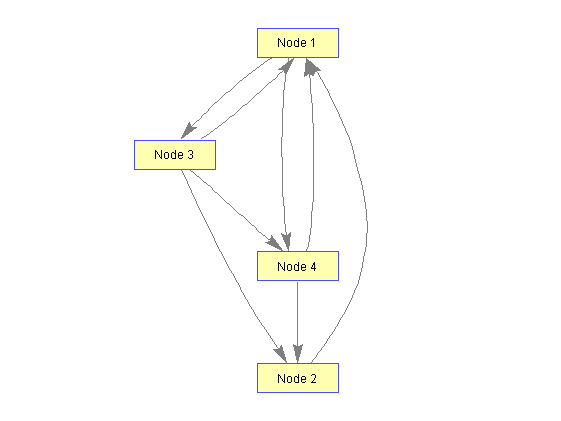
\includegraphics[scale=0.45]{../images/a1_graph.png}\label{fig:a1_graph}
	\caption{Graphe de $A_1$}
\end{figure}
\paragraph{2)} Avant de calculer la matrice de transition, il est nécessaire de caractériser la marche aléatoire. Autrement dit, il faut définir les poids/probabilités que nous appliquerons aux arêtes du graphe sur lequel le surfeur va évoluer. Nous avons déduit de l'énoncé du projet que les différentes possibilités de quitter un nœud devaient être \textbf{équiprobables} et nous utiliserons donc cette hypothèse dans la suite du rapport.
\paragraph{}
Suite à ce choix, la formation de la matrice de transition est très simple. Si l'on note $A$ la matrice d'adjacence, alors il suffit d'appliquer la formule suivante pour calculer l'élément $Q(i,j)$ :
\[
Q(i,j) = A(i,j) \times \frac{1}{n}\sum\limits_{j = 1}^n A(i,j)
\]
Cette formule permet de placer à $0$ les éléments de $Q$ représentant une transition impossible et de placer à une certaine probabilité les autres éléments de $Q$ (toute probabilité non nulle d'une ligne de Q étant équiprobable comme attendu). Nous avons représenté le diagramme d'états à la \textsc{Figure} \ref{fig:Q1}

\begin{figure}[h]
	\center
	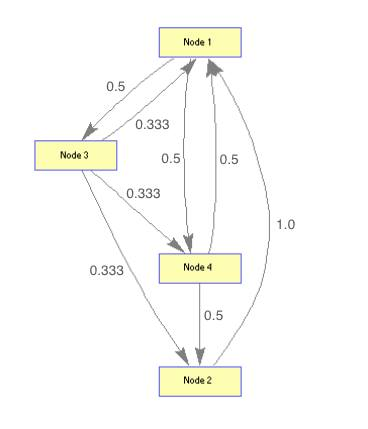
\includegraphics[scale=0.45]{../images/Q1.jpg}\label{fig:Q1}
	\caption{Diagramme d'états à partir de $A_1$}
\end{figure}

\paragraph{3)} Nous avons choisi un nombre de pas $t = 20$. Le cas où le surfeur démarre aléatoirement sur le graphe est représenté par une distribution initiale $\pi_0$ uniforme et le cas où il démarre d'une page fixe est représenté par une distribution initiale $\pi_0$ où toutes les probabilités sont nulles sauf celle située l'index correspondant au nœud de départ. L'évolution des probabilités dans les deux cas est donnée sur le \textsc{Figure} \ref{fig:q113}.
\begin{figure}[h]
	\center
	\subfigure{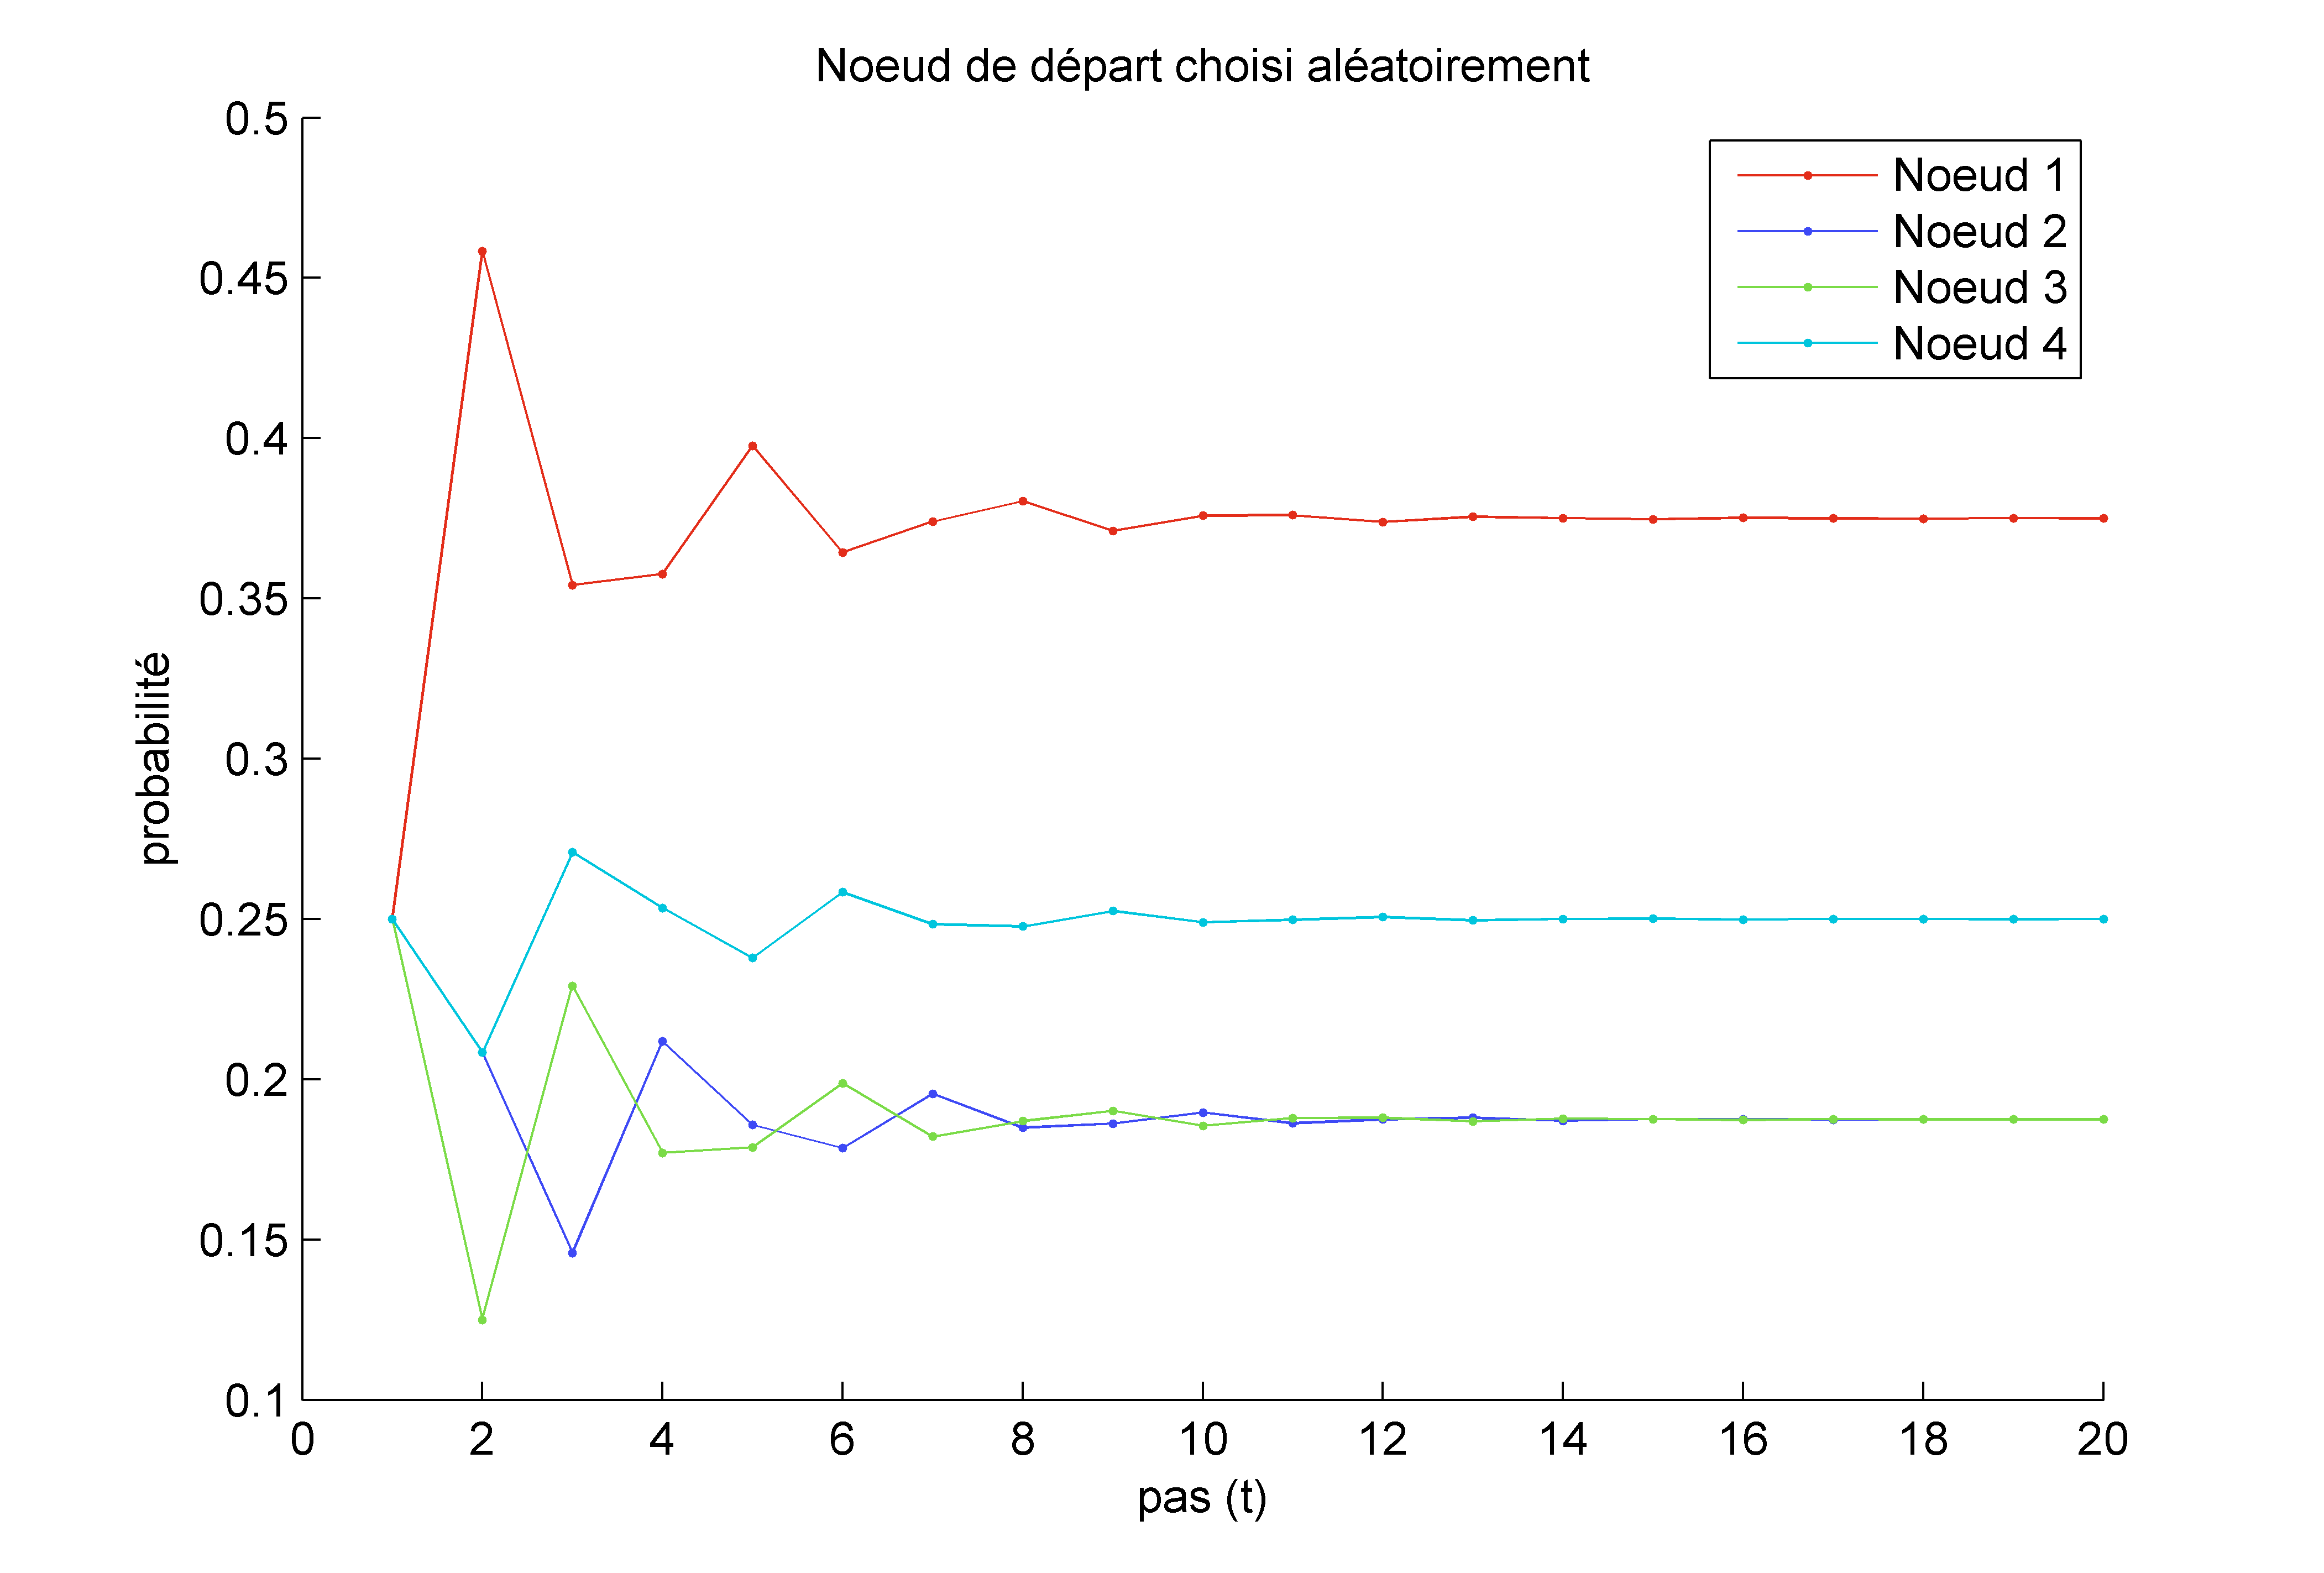
\includegraphics[scale=0.4]{../images/q1131_proba.png}}
	\subfigure{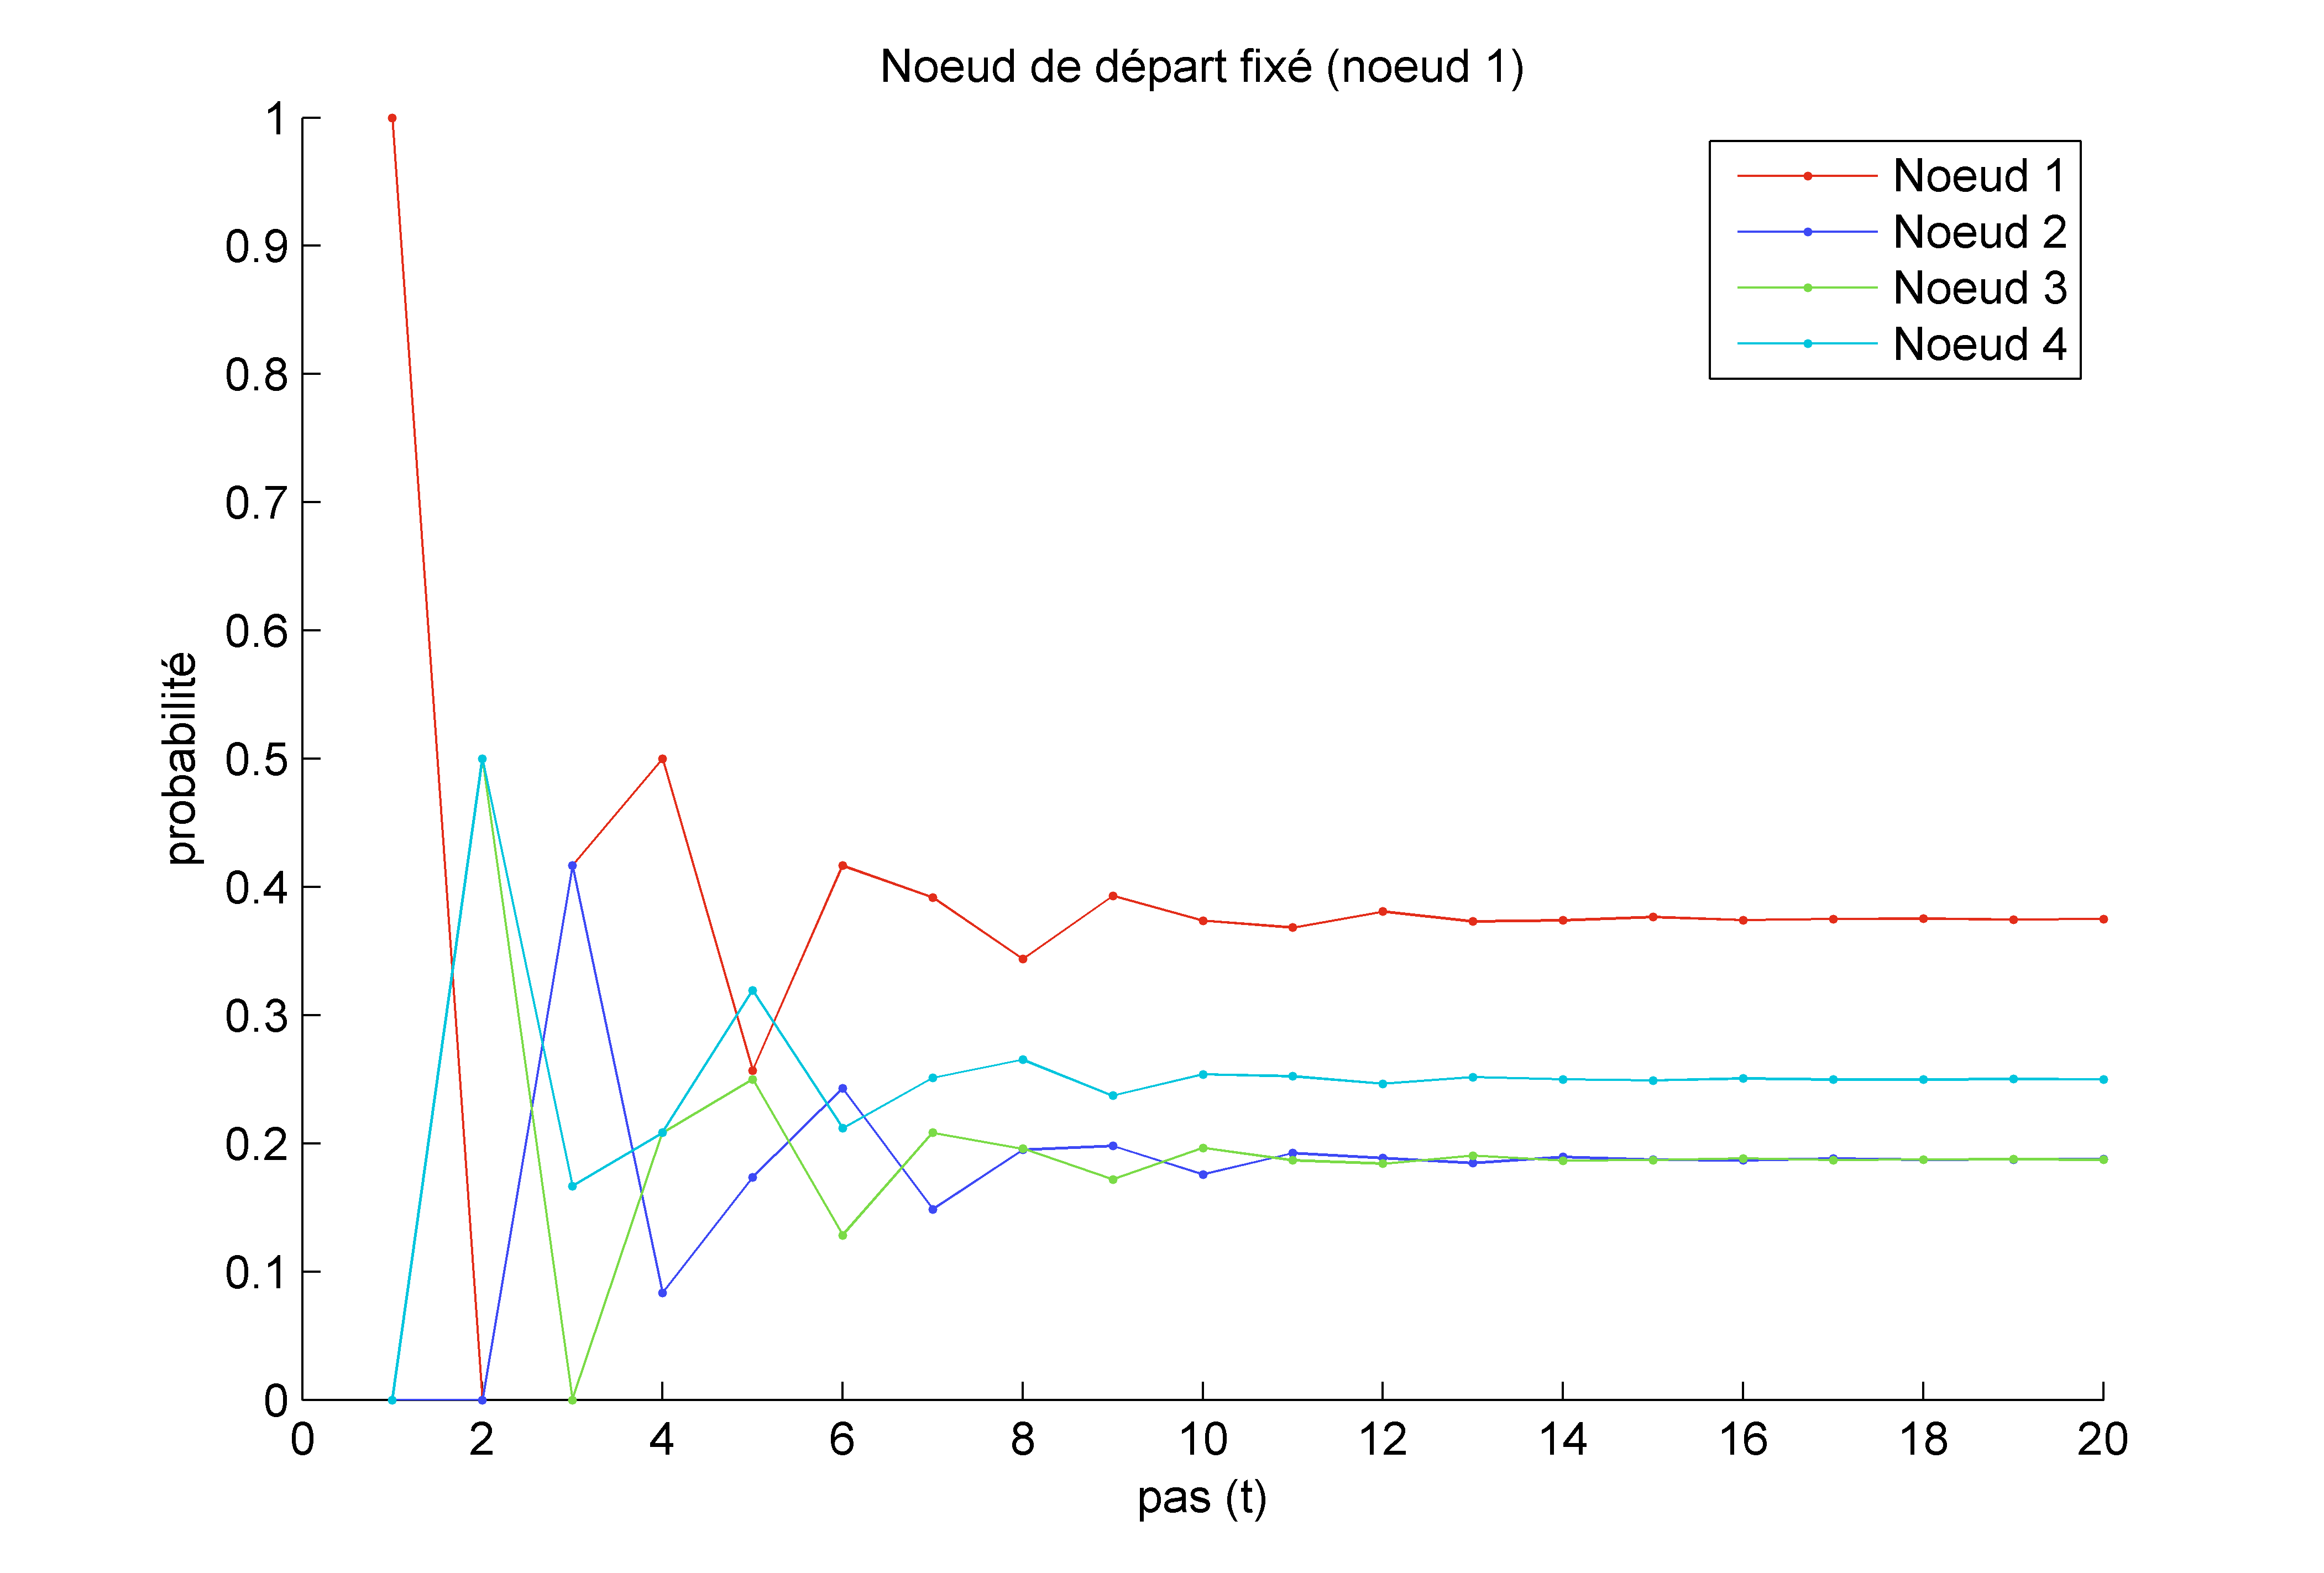
\includegraphics[scale=0.4]{../images/q1132_proba.png}}
	\caption{Évolution de la distribution de probabilité}
	\label{fig:q113}
\end{figure}
\paragraph{}
La matrice $Q^{(20)}$ obtenue est la suivante :
\[
Q^{(20)} = 
\begin{pmatrix}
 0.3751 & 0.1874 & 0.1875 & 0.2500\\
 0.3751 & 0.1877 & 0.1874 & 0.2499\\
 0.3749 & 0.1875 & 0.1875 & 0.2500\\
 0.3749 & 0.1875 & 0.1875 & 0.2500\\
\end{pmatrix}
\]
Si on observe les matrices $Q^{(k)}$ pour $k> 20$, on peut constater que les éléments se stabilisent et que les lignes s'égalisent. 
\paragraph{4)} La distribution stationnaire a été calculée par la méthode des puissances. Nous avons donc multiplié les distributions $\pi^{(k)}$ successives par $Q$ jusqu'à ce que cette distribution se stabilise. Le critère de stabilisation choisi était le suivant : 
\[
\max\left(\left|\pi_j^{(k)} - \pi_j^{(k - 1)}\pi\right|\right) < \varepsilon
\]
où $\pi_j$ est la $j^{\text{ième}}$ composante du vecteur $\pi$. La distribution stationnaire obtenue est donnée ci-dessous :
\[
\pi_\infty = 
\begin{pmatrix}
0.3750 &
0.1875 &
0.1875 &
0.2500 \\
\end{pmatrix}
\]
On constate que les lignes de la matrice sont très proches des valeurs observables sur les graphiques du point précédent.
\paragraph{5)} On constate que le nœud 1 possède le meilleur PageRank, suivi des nœuds 2 et 3 à égalité et du nœud 4. On peut expliquer ce classement intuitivement : 
\begin{itemize}
	\item le \textbf{nœud 1} possède le plus d'arêtes entrantes donc ayant le plus de chance d'être visité
	\item le \textbf{nœud 3} possède le moins d'arêtes entrantes donc ayant le moins de chance d'être visité
	\item les \textbf{nœuds 2} et \textbf{4} possèdent le même nombre intermédiaire (par rapport aux deux autres) d'arêtes entrantes. Le PageRank du nœud 4 est néanmoins plus élevé que celui du nœud 2 puisque le nœud 4 possèdent une arête entrante venant du nœud 1 qui est le plus visité.
	\item malgré un nombre d'arêtes entrantes plus élevé que pour le nœud 3, le \textbf{nœud 2} possède une PageRank égal. Cela est dû au fait que, d'une part, le nœud 3 peut être visité depuis le nœud le plus visité (nœud 1) ce qui améliore son PageRank et, d'autre part, que le nœud 2 ne peut être accédé depuis des nœuds moins visités (nœud 3 et 4) ce qui abaisse son PageRank. 
\end{itemize} 
\paragraph{6)} Dans un premier temps, nous avons généré une chaîne pour chaque longueur. Le résultat obtenu est donné sur la Figure \ref{sfig:q116_evol_1}. On peut déjà observer que les différentes courbes obtenues oscillent autour de leur probabilité stationnaire correspondante. Néanmoins, étant donné la présence d'oscillations, nous avons décidé de refaire l'expérience en générant cette fois-ci 1000 chaînes pour chaque longueur. Nous avons ensuite moyenné les différentes probabilités afin d'obtenir un résultat plus précis (voir Figure \ref{sfig:q116_evol_2}). Les courbes obtenues nous permettent de confirmer les premières observations.
\paragraph{}
Remarquons aussi que, quelque soit la distribution de départ, la distribution converge vers la distribution stationnaire.
\begin{figure}[h]
	\center
	\subfigure[1 génération]{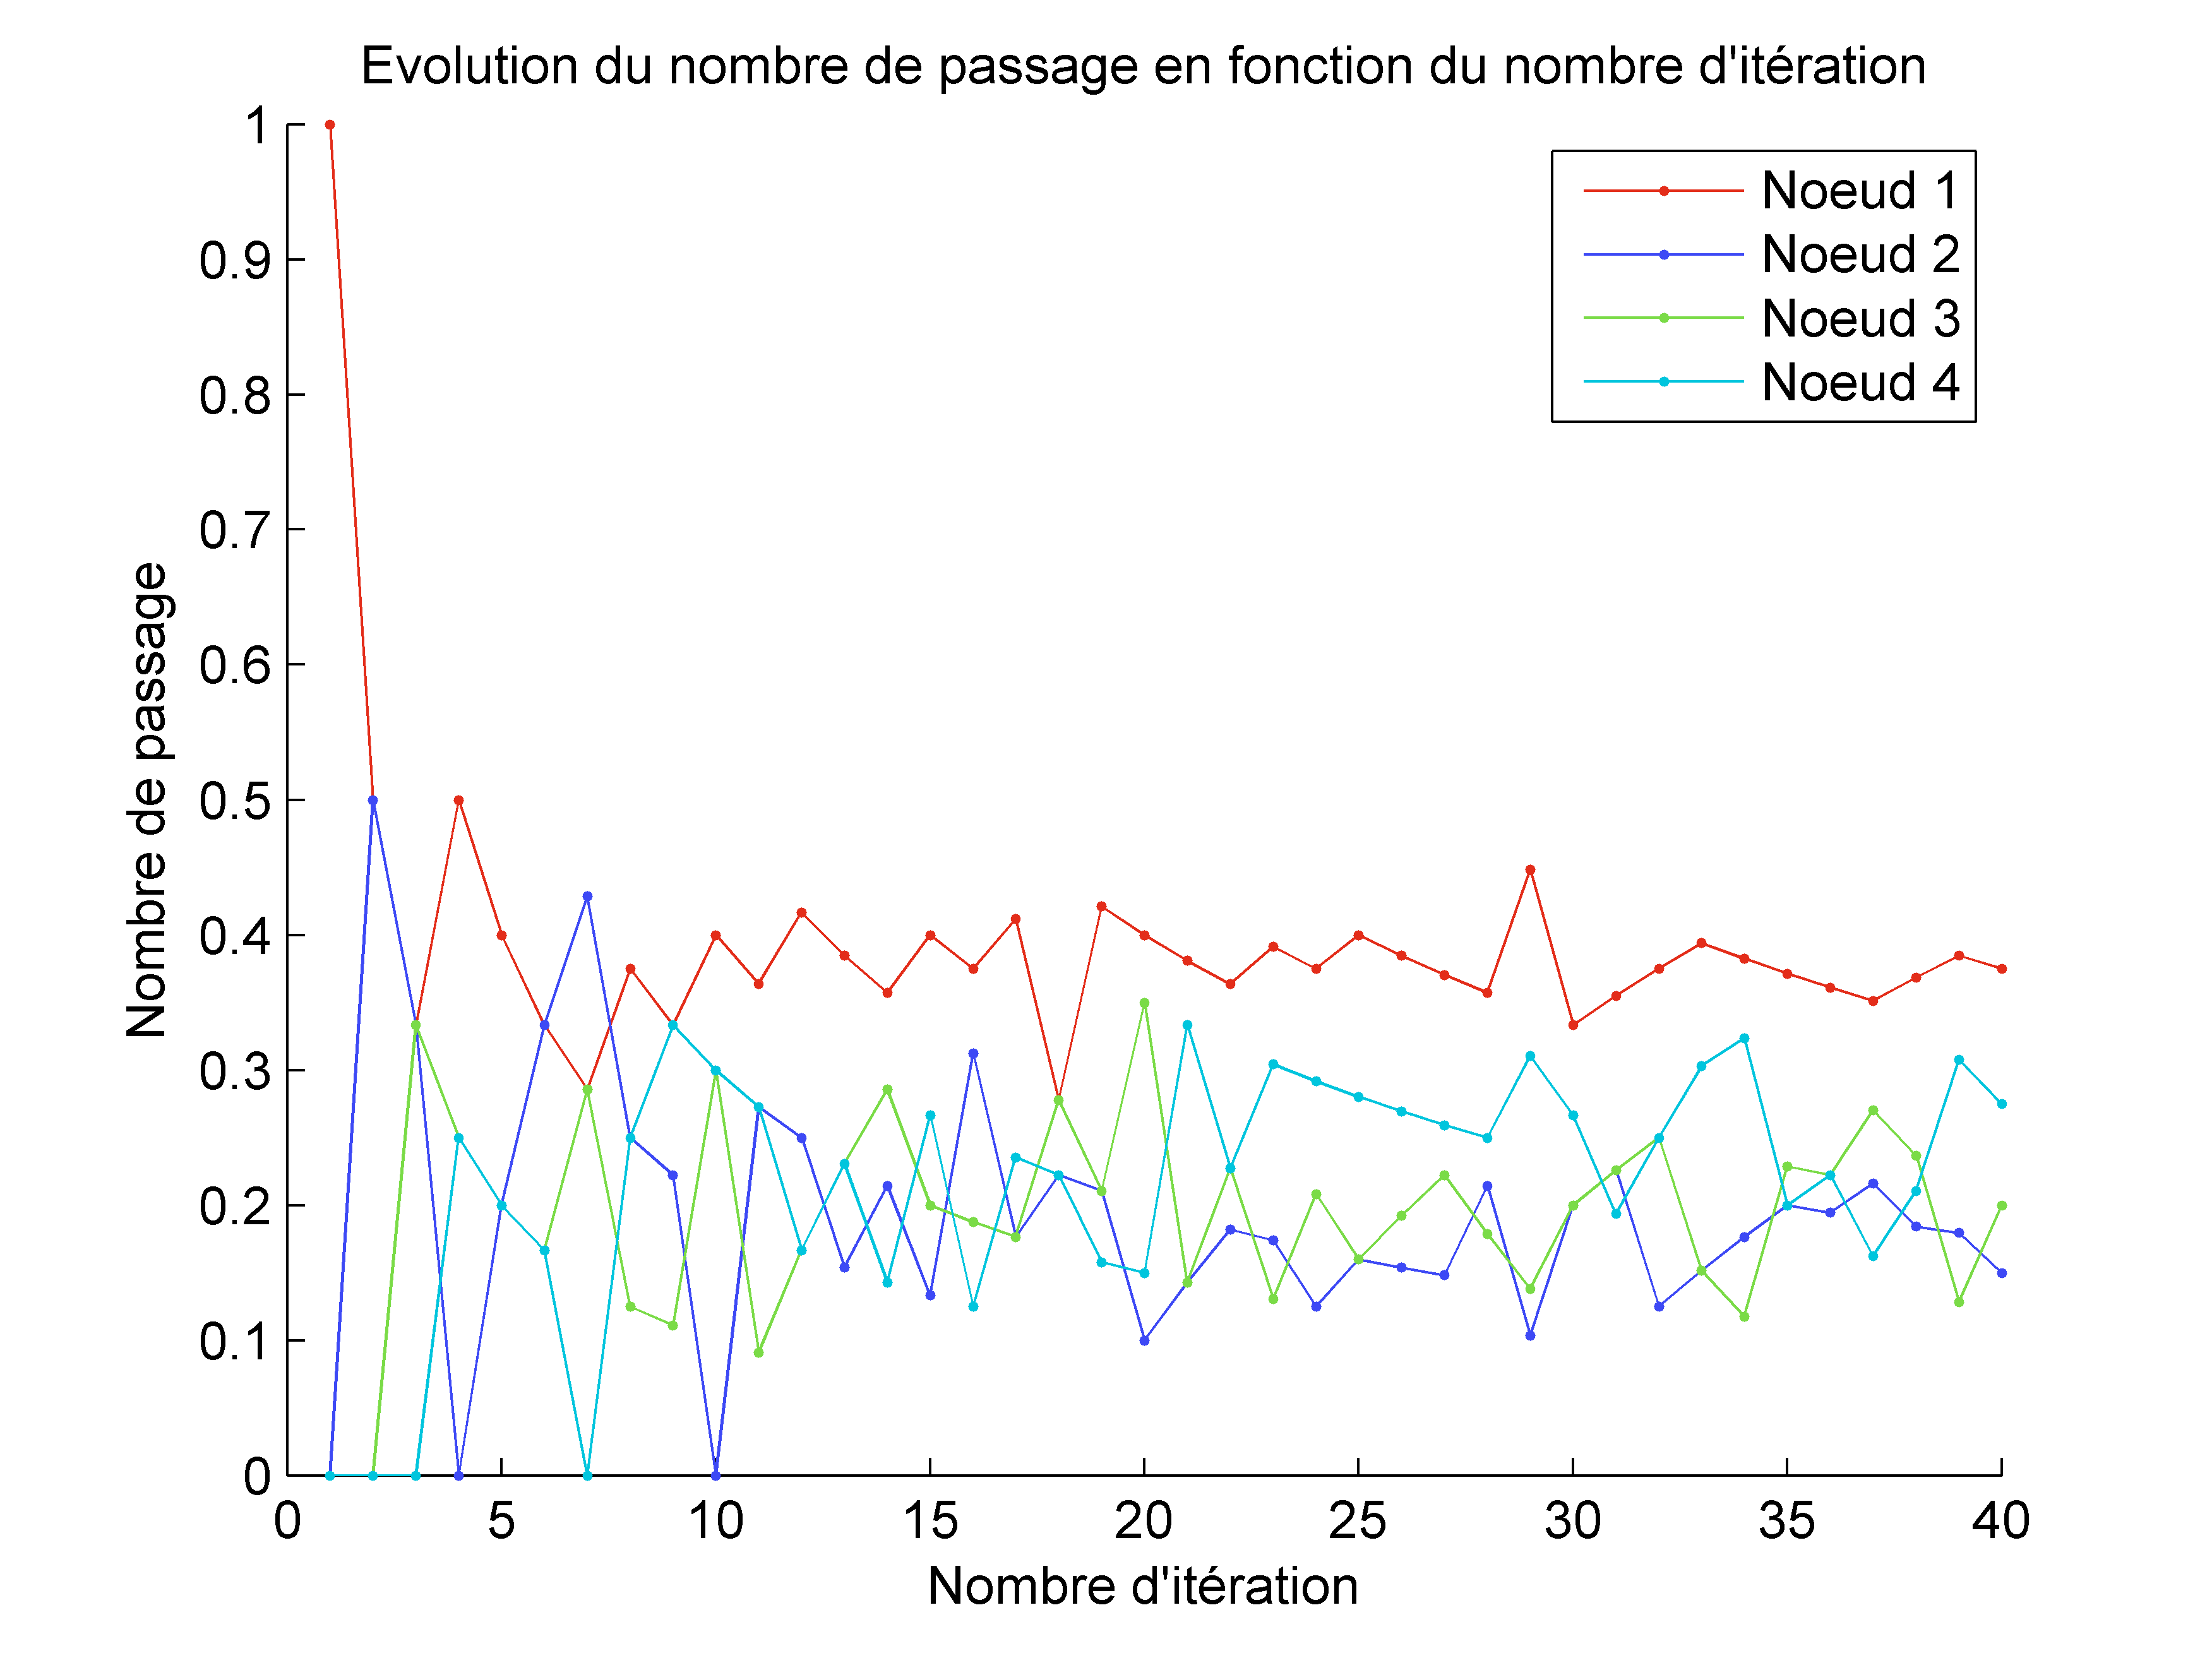
\includegraphics[scale=0.47]{../images/q116_evol_1.png}\label{sfig:q116_evol_1}}
	\subfigure[1000 générations]{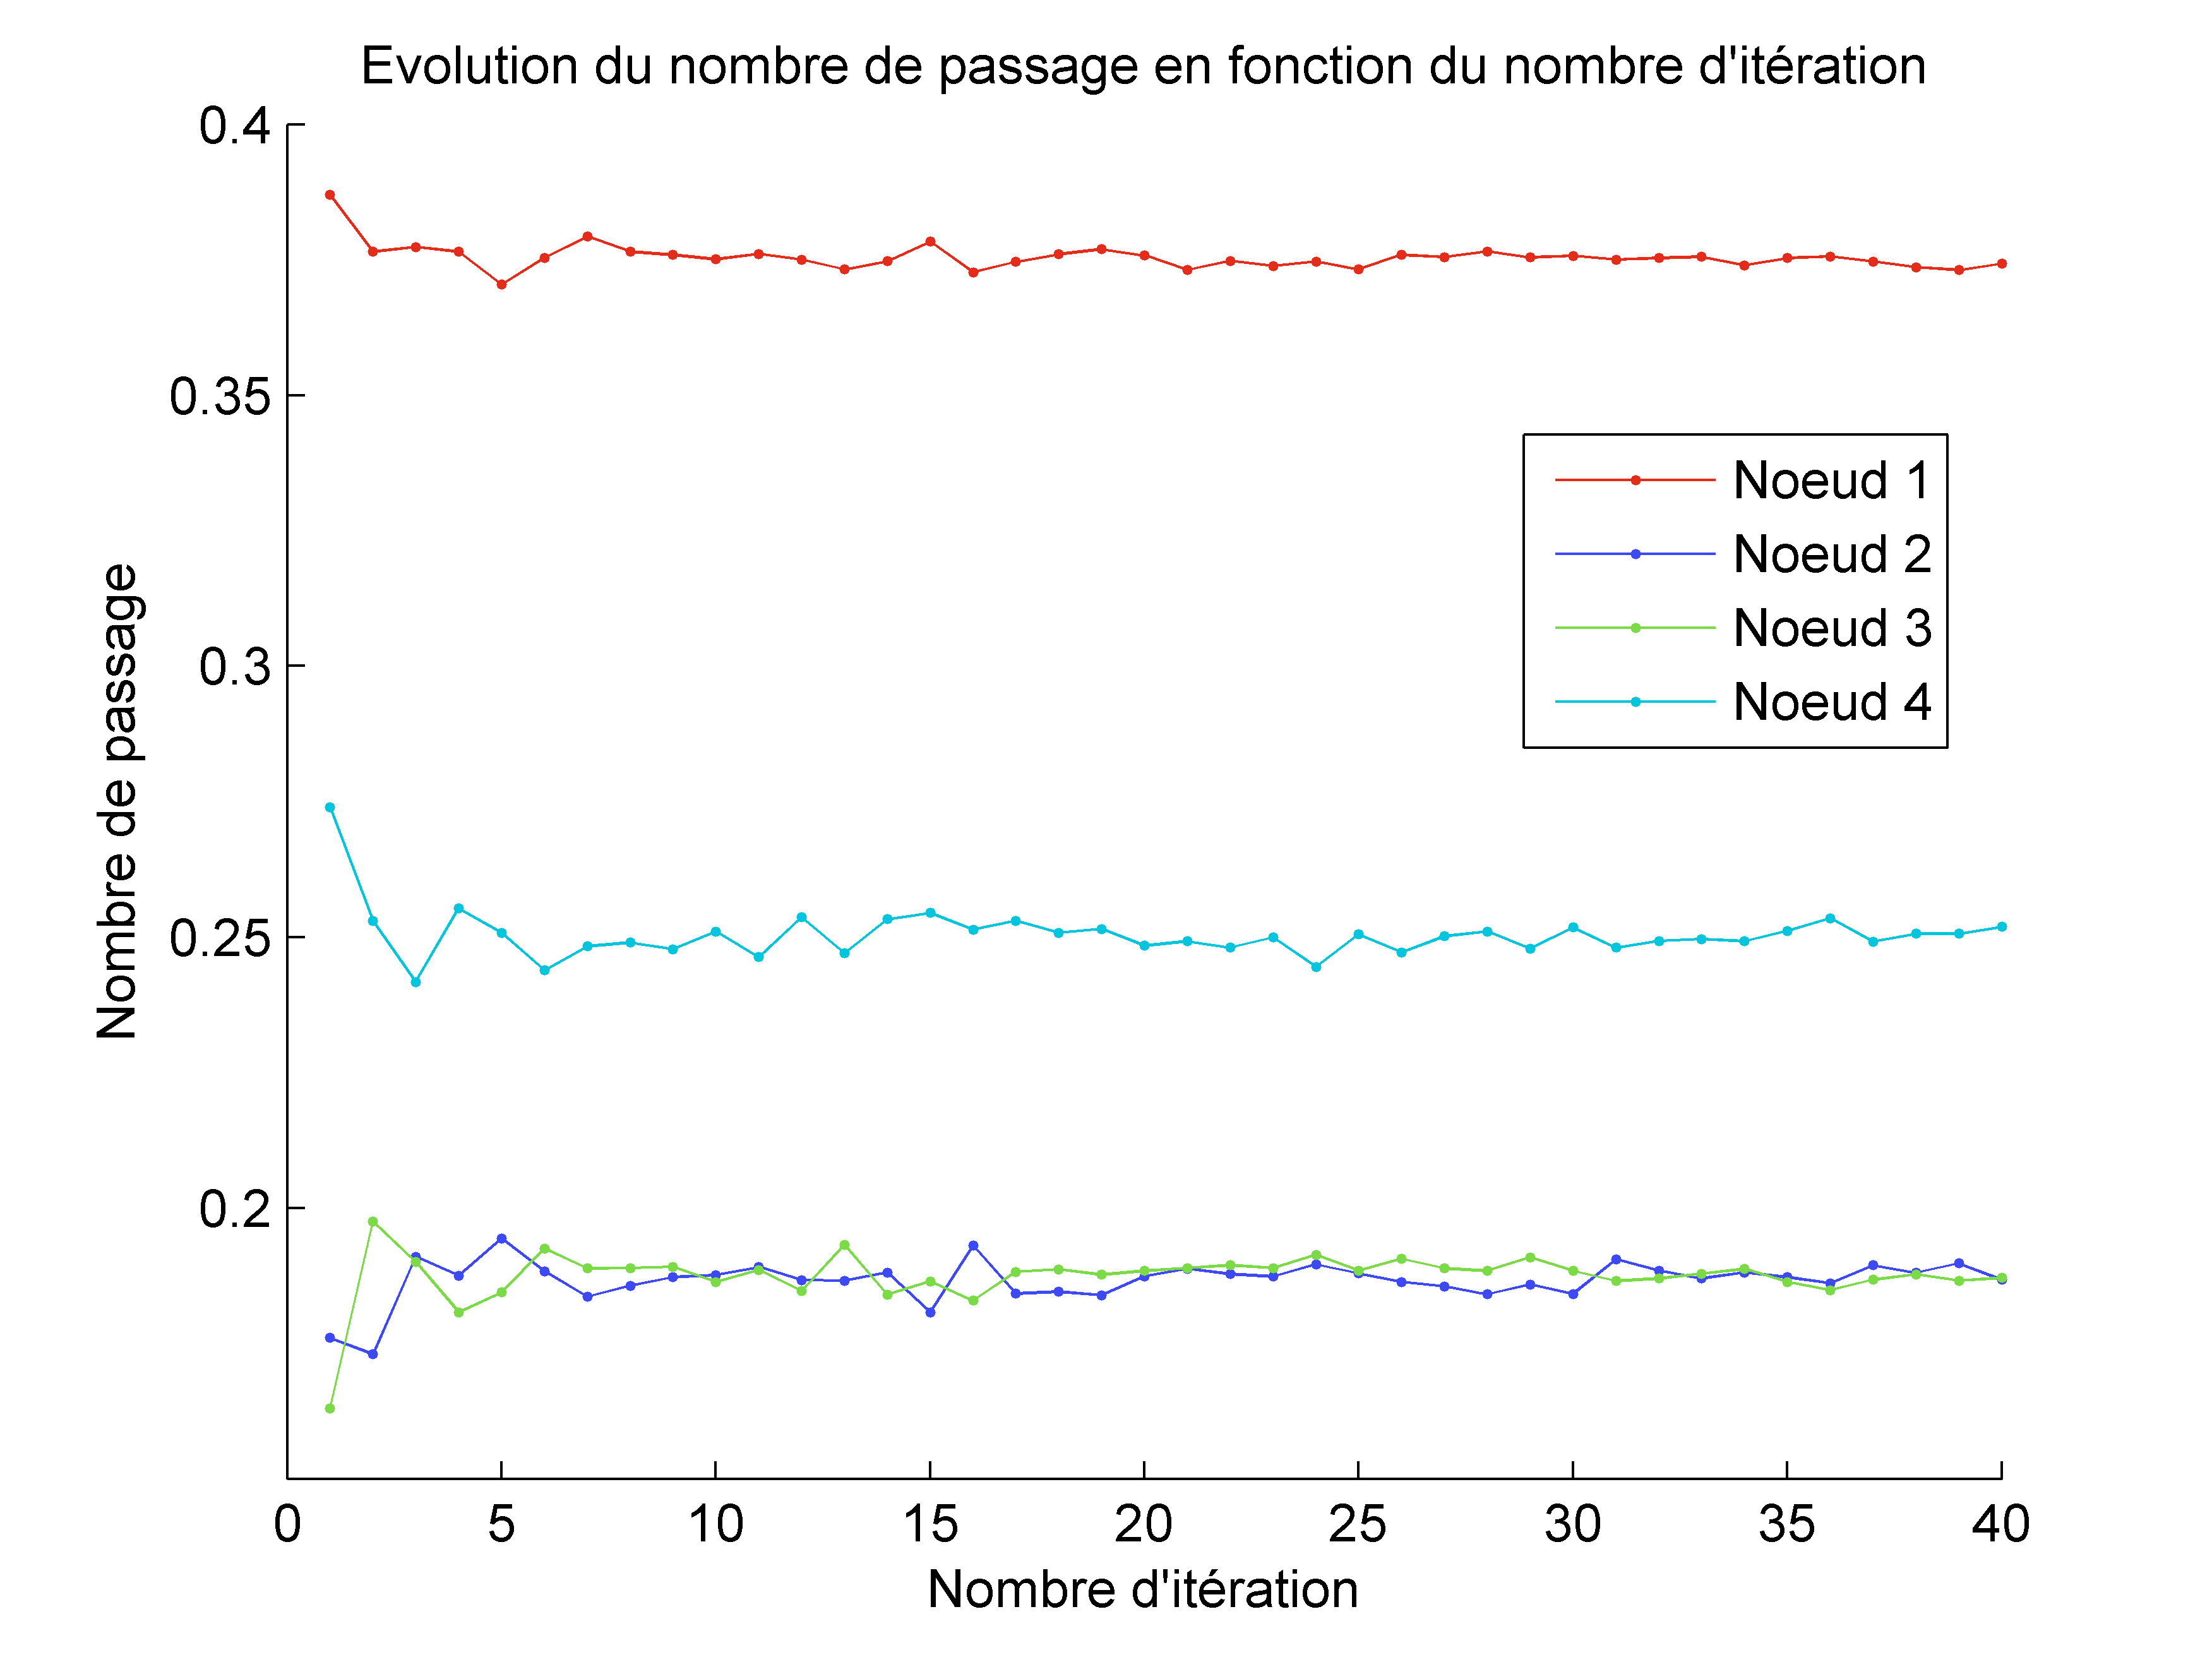
\includegraphics[scale=0.47]{../images/q116_evol_2.png}\label{sfig:q116_evol_2}}
	\caption{Évolution du nombre de passage par un nœud}
\end{figure}
\paragraph{7)} 
Nous pouvons relier ces résultats à la théorie car la chaîne est \textbf{\textit{ergodique}}. En effet : \\
\begin{itemize}
\item[•] Premièrement, la chaîne est \textbf{\textit{irréductible}} car il est possible de visiter tous les autres nœuds à partir de n'importe quel nœud donné.
\item[•] Deuxièmement, la chaîne est \textbf{\textit{apériodique}} car le plus grand commun diviseur du nombre de pas nécessaires \textbf{N} pour aller d'un nœud vers lui même est inférieur à 2. Si on analyse le graphe, on observe que pour les nœuds 1, 3 et 4 le nombre de pas nécessaires vaut 2 alors que ce nombre vaut trois pour le nœud 2. \textbf{N} vaut donc 1.\\
\end{itemize}

Dans l'expérience du point 6, nous avons observé que la distribution de probabilité stationnaire correspond aux probabilités trouvées sur nos graphes lorsque le nombre d'itérations est assez élevé.


\subsection*{Analyse des graphes $A_2$ et $A_3$}
\paragraph{1)} Pour pouvoir calculer des éventuelles distributions stationnaires sur base des matrices $A_2$ et $A_3$, nous avons calculé les matrices de transition $Q_2$ et $Q_3$ : 
\[
Q_2 = 
\begin{pmatrix}
         0 &   1.0000  &       0  &       0 \\
         0 &        0  &       0  &  1.0000 \\
    0.5000 &   0.5000  &       0  &       0 \\
    1.0000 &        0  &       0  &       0 \\
\end{pmatrix}
\,\,
Q_3 = 
\begin{pmatrix}
        0  &   1.0000   &      0  &       0  &       0 \\
    1.0000 &        0   &      0  &       0  &       0 \\
         0 &   0.3333   &      0  &  0.3333  &  0.3333 \\
         0 &        0   &      0  &       0  &  1.0000 \\
         0 &        0   &      0  &  1.0000  &       0 \\
\end{pmatrix}
\]
Nous avons représenté les diagrammes d'états des deux chaînes de Markov sur la \textsc{Figure} \ref{fig:Q23}. 
\begin{figure}[h]
	\center
	\subfigure{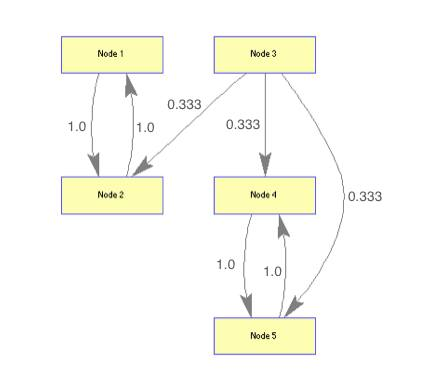
\includegraphics[scale=0.45]{../images/Q2.jpg}}
	\subfigure{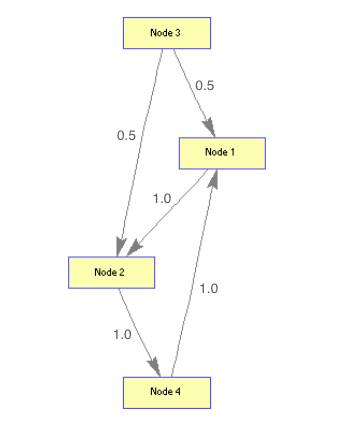
\includegraphics[scale=0.45]{../images/Q3.jpg}}
	\caption{Diagramme d'état de $A_2$ et $A_3$}
	\label{fig:Q23}
\end{figure} 
Nous avons ensuite appliqué la méthode des puissances pour obtenir des distributions $\pi^{(k)}$ successives. Le résultat est donné sur la \textsc{Figure} \ref{fig:q118}. On constate qu'aucune distribution stationnaire n'a pu être trouvée étant donné la présence d'\textbf{oscillations}.
\paragraph{}
On constate aussi que la \textbf{probabilité} d'atteindre une certain nœud \textbf{tombe à 0} ou est directement nulle dès la première itération dans les deux situations. Ce phénomène est dû à la présence de \textit{dangling nodes} dans les deux graphes. On peut directement voir la présence de ce type de nœud sur les matrices de transitions : elle se manifeste par une colonne composée uniquement de probabilités nulles et implique qu'il est impossible de passer d'un nœud quelconque au \textit{dangling node}.
\paragraph{}
Ces deux phénomènes sont précisément des \textbf{limitations} du modèle du surfeur aléatoire simpliste présenté dans cette première partie. D'une part, les oscillations empêchent d'atteindre une distribution stationnaire. D'autre part, la probabilité nulle d'atteindre un nœud existant rend l'éventuelle distribution stationnaire (et donc le PageRank) peu représentative de l'organisation des nœuds puisqu'elle omet d'en prendre certains en compte.
\paragraph{}
Les \textbf{causes de ces phénomènes} sont d'une part la présence d'un cycle infini dans les graphes et la présence de \textit{dangling nodes}. Ces problèmes vont être contournés en introduisant la téléportation dans la section suivante.
\begin{figure}[h]
	\center
	\subfigure[Distribution initiale uniforme]{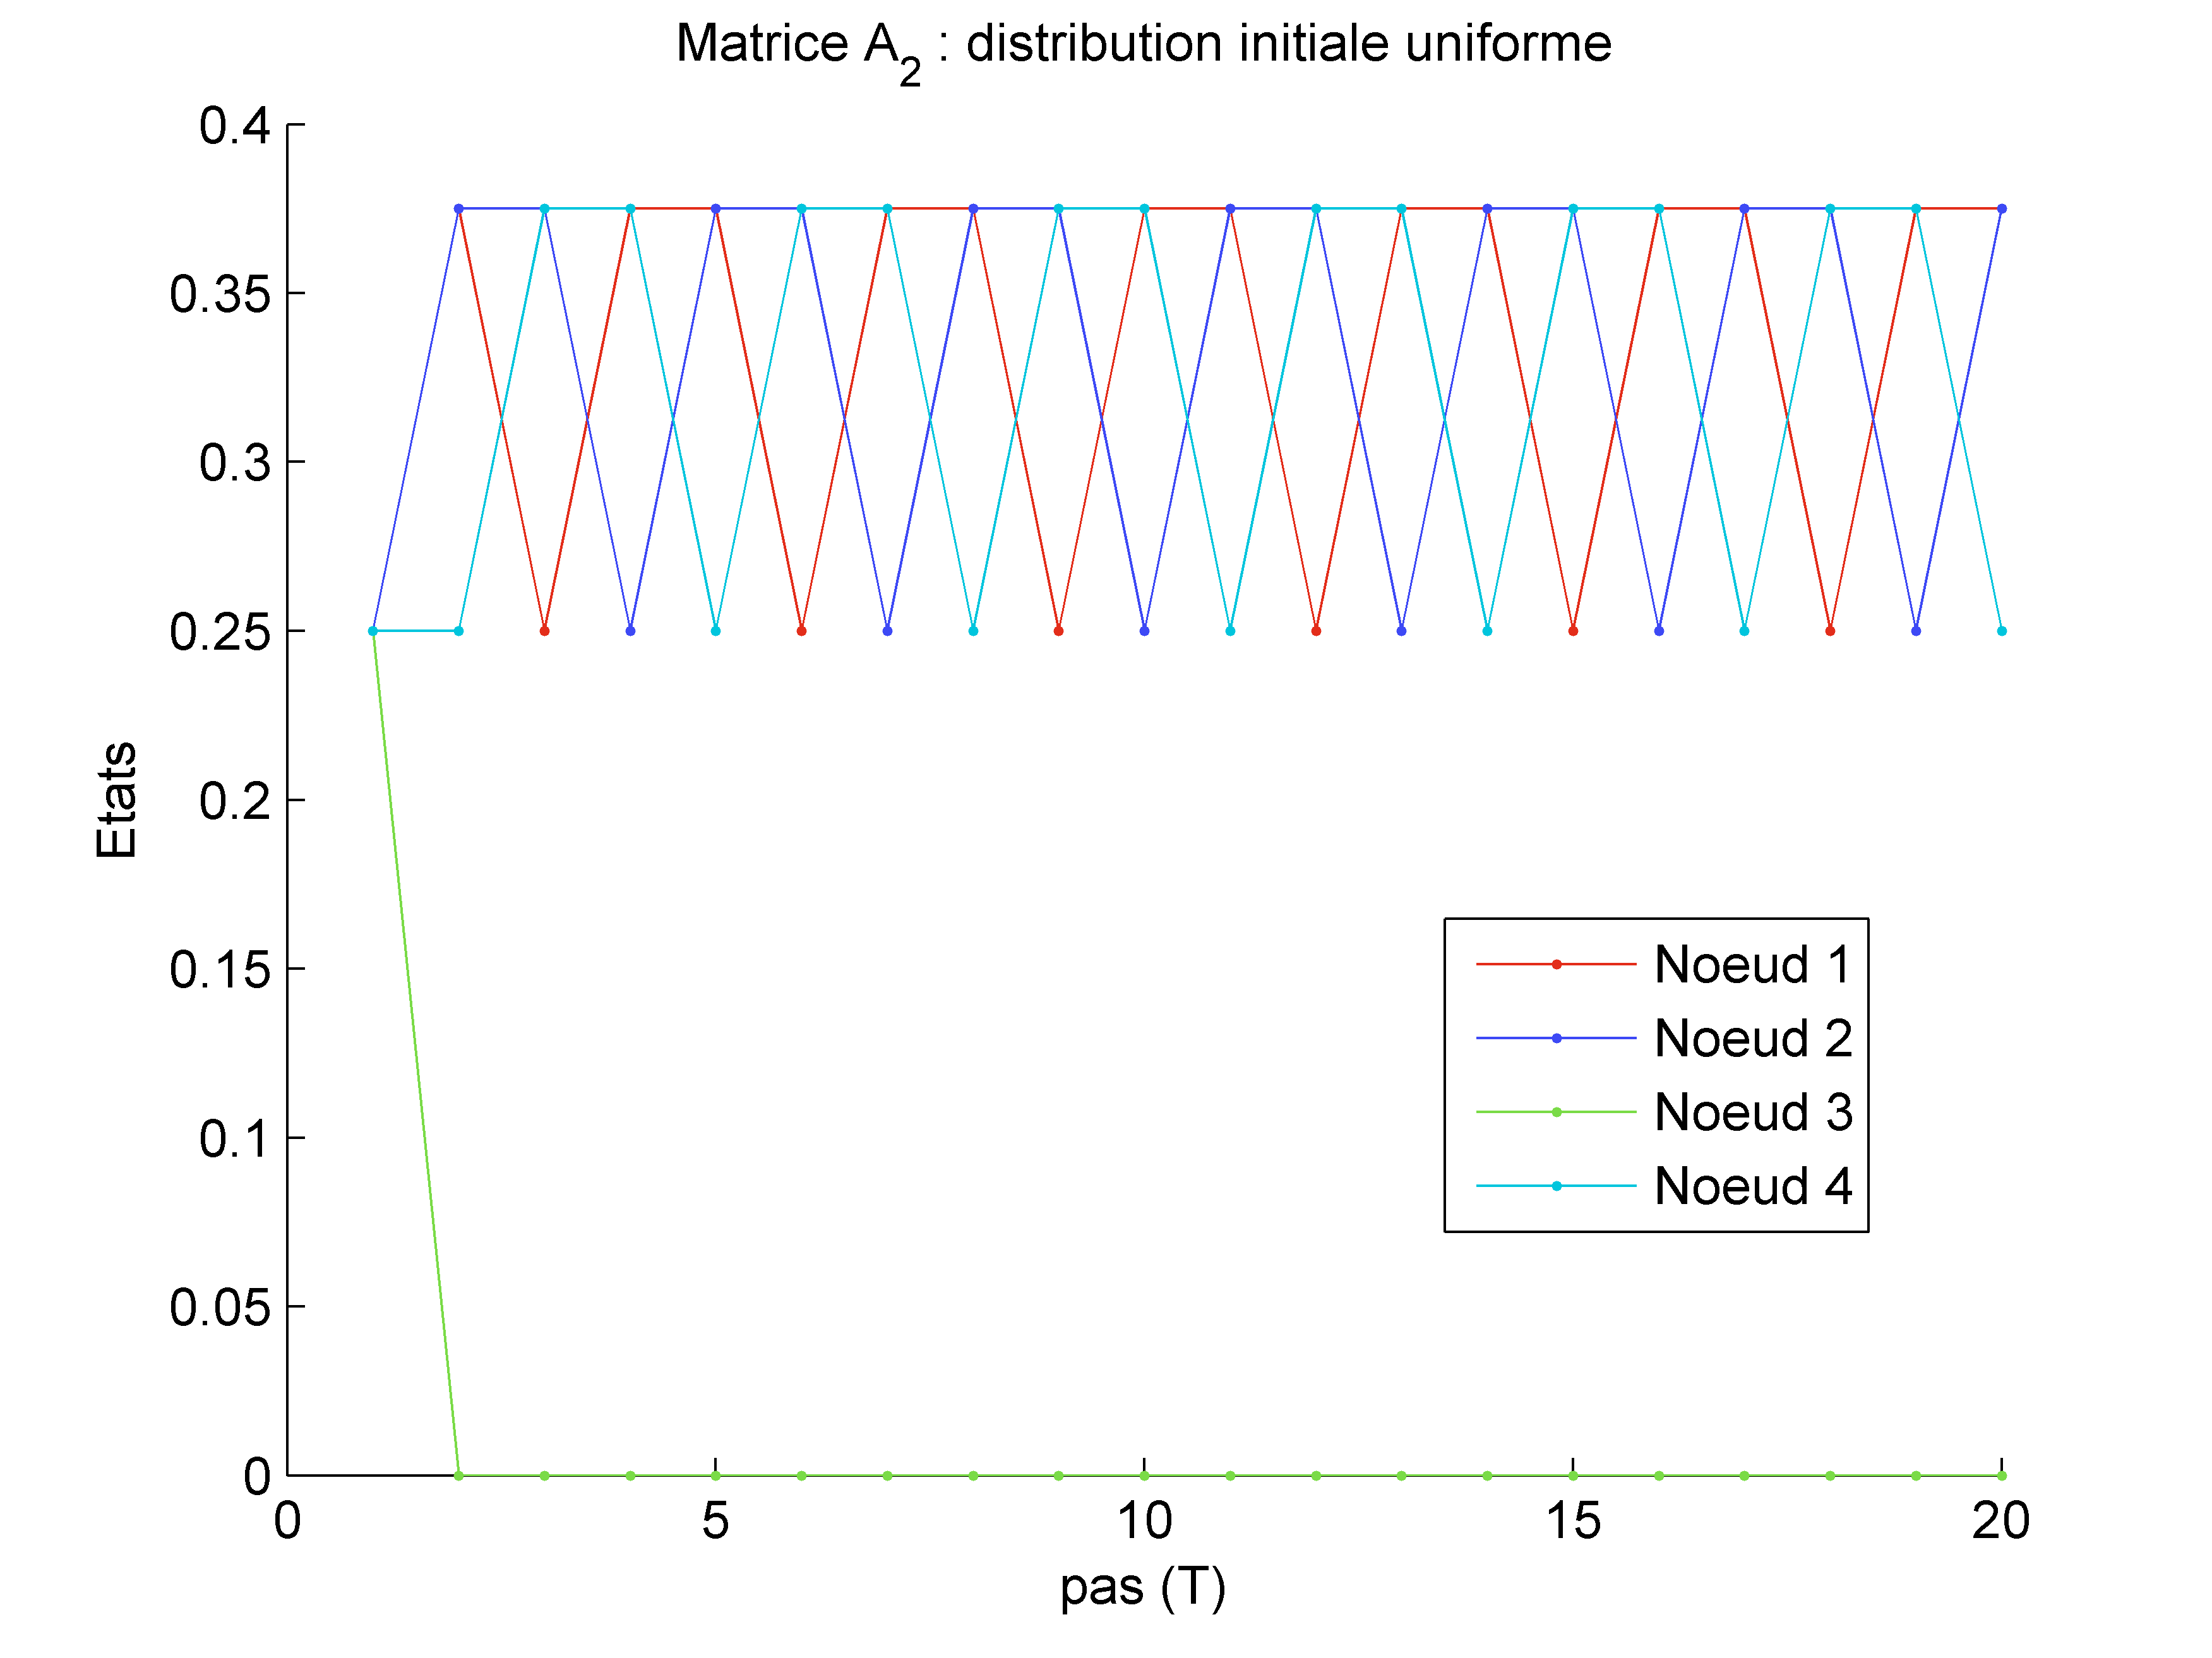
\includegraphics[scale=0.45]{../images/q118_evol_21.png}\label{sfig:q118_evol}}
	\subfigure[Depuis le noeud 1]{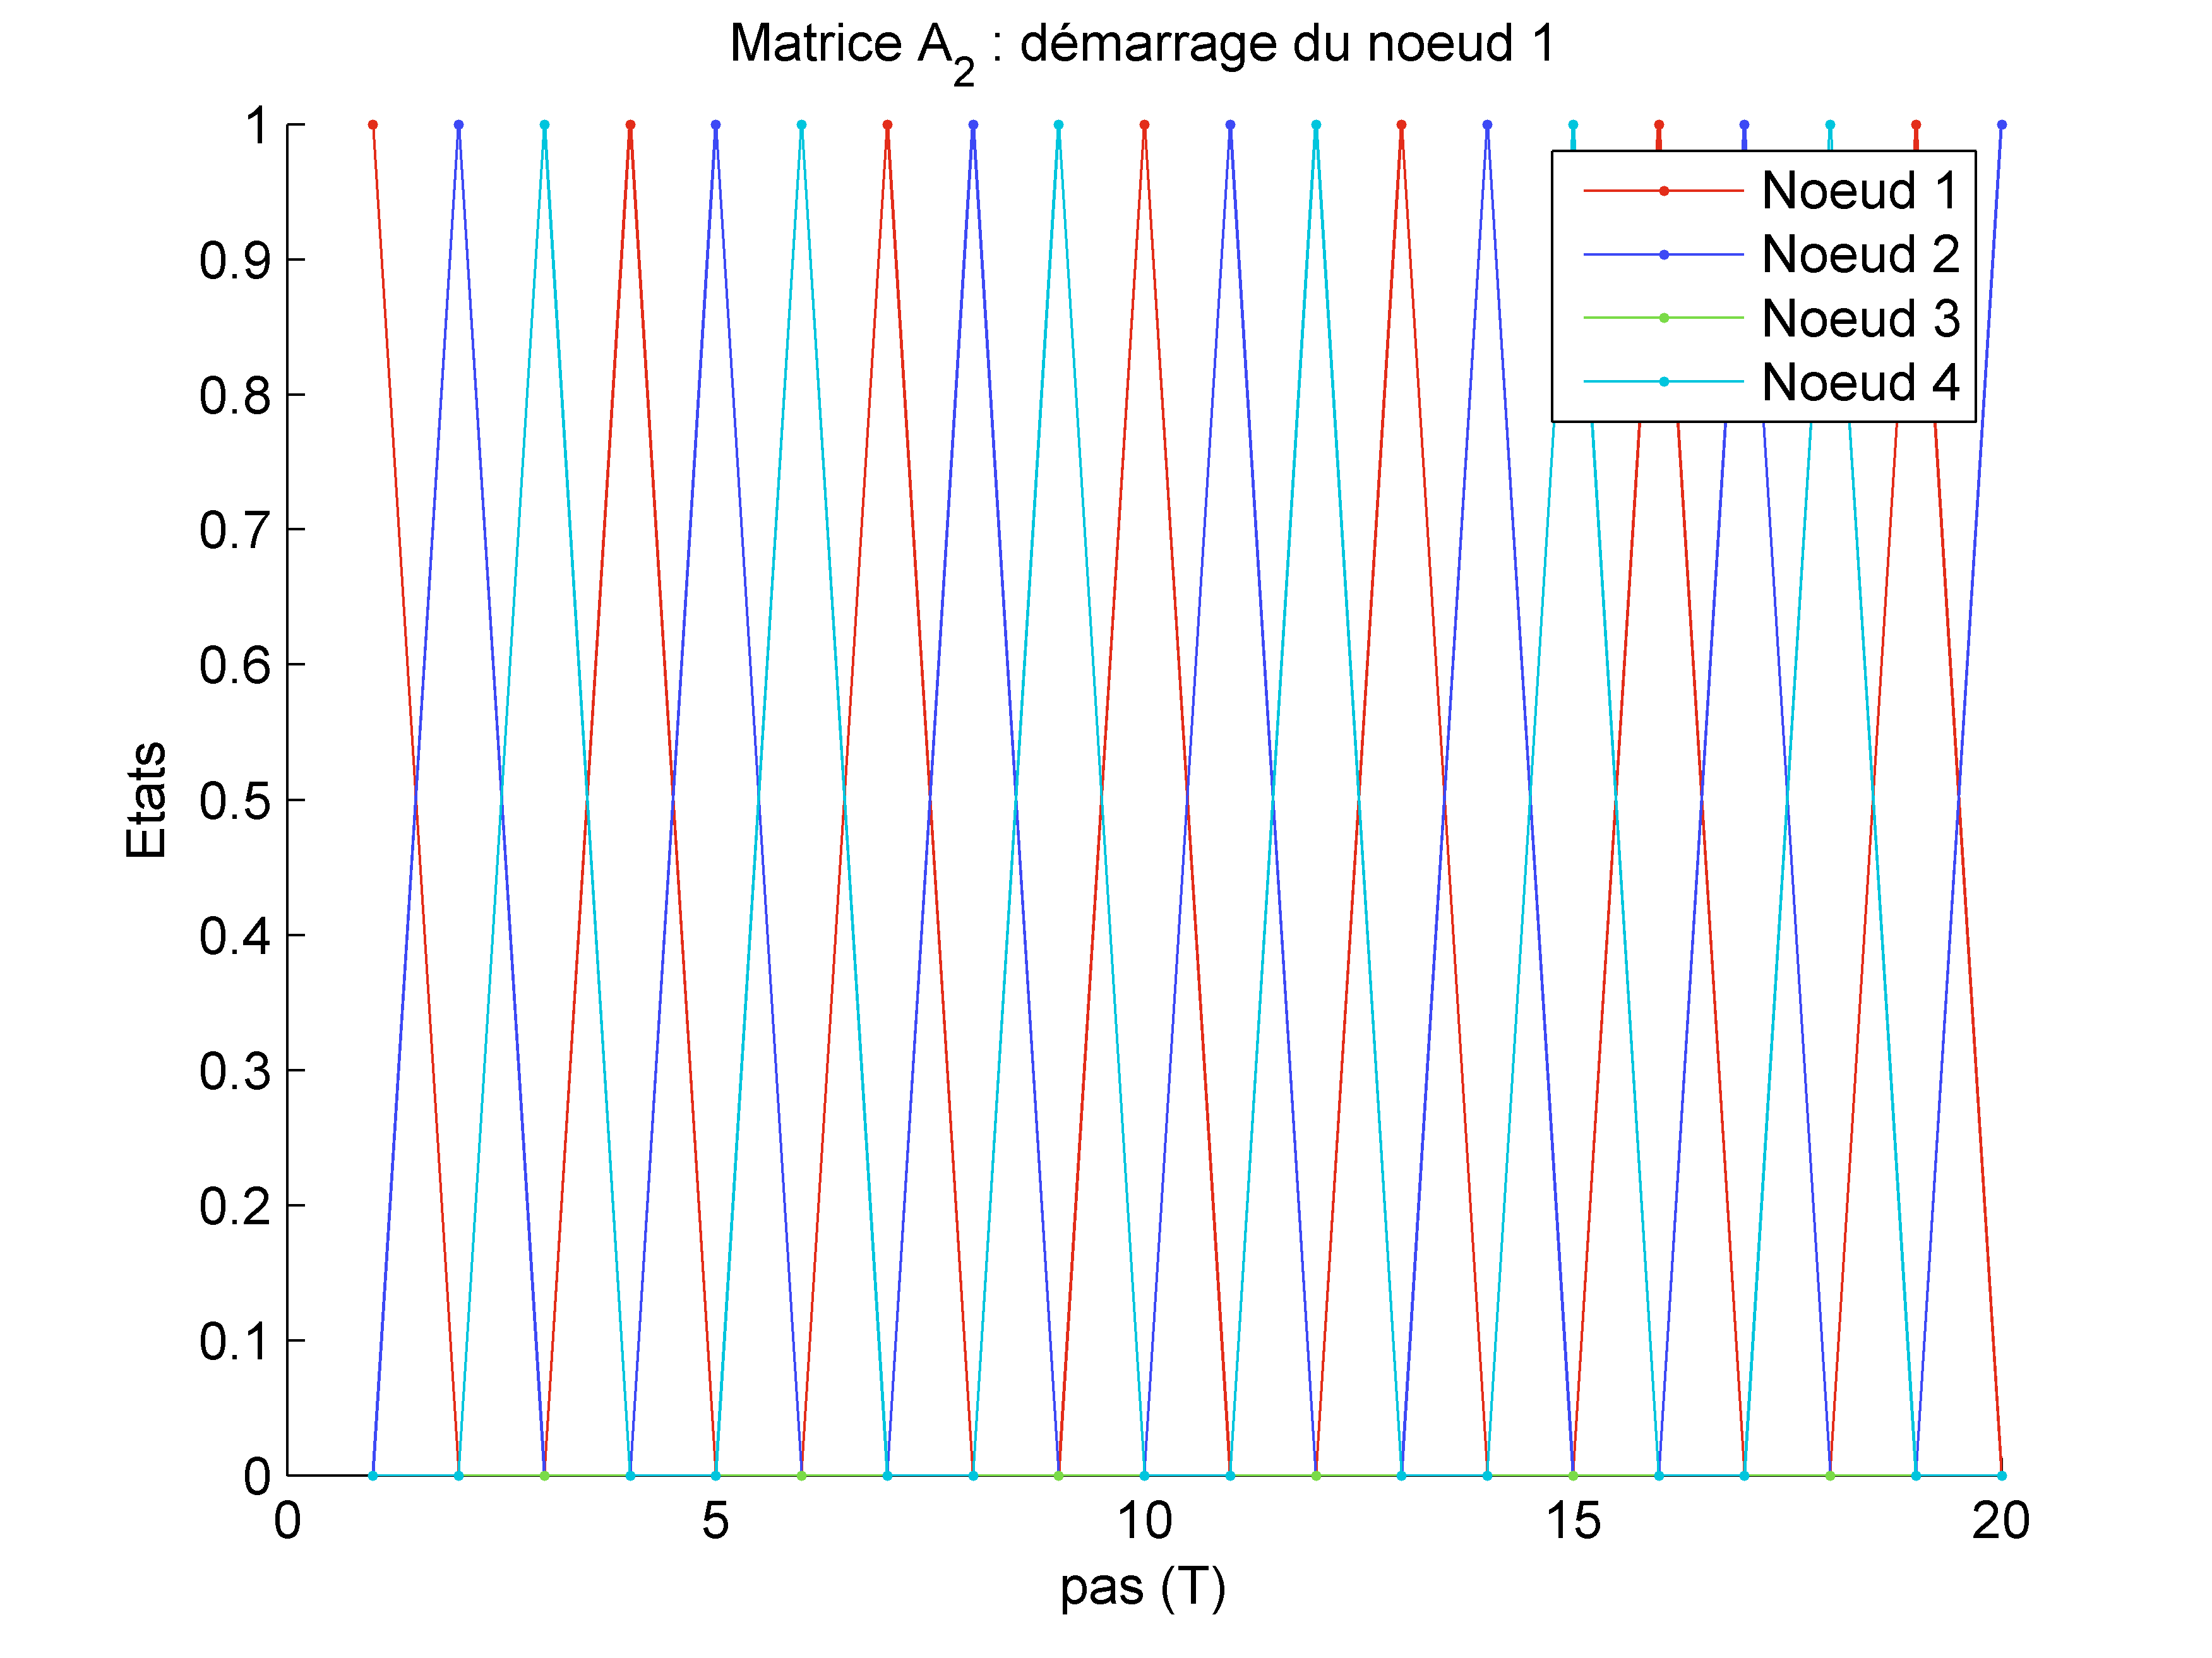
\includegraphics[scale=0.45]{../images/q118_evol_22.png}\label{sfig:q118_evol}}
	\subfigure[Distribution initiale uniforme]{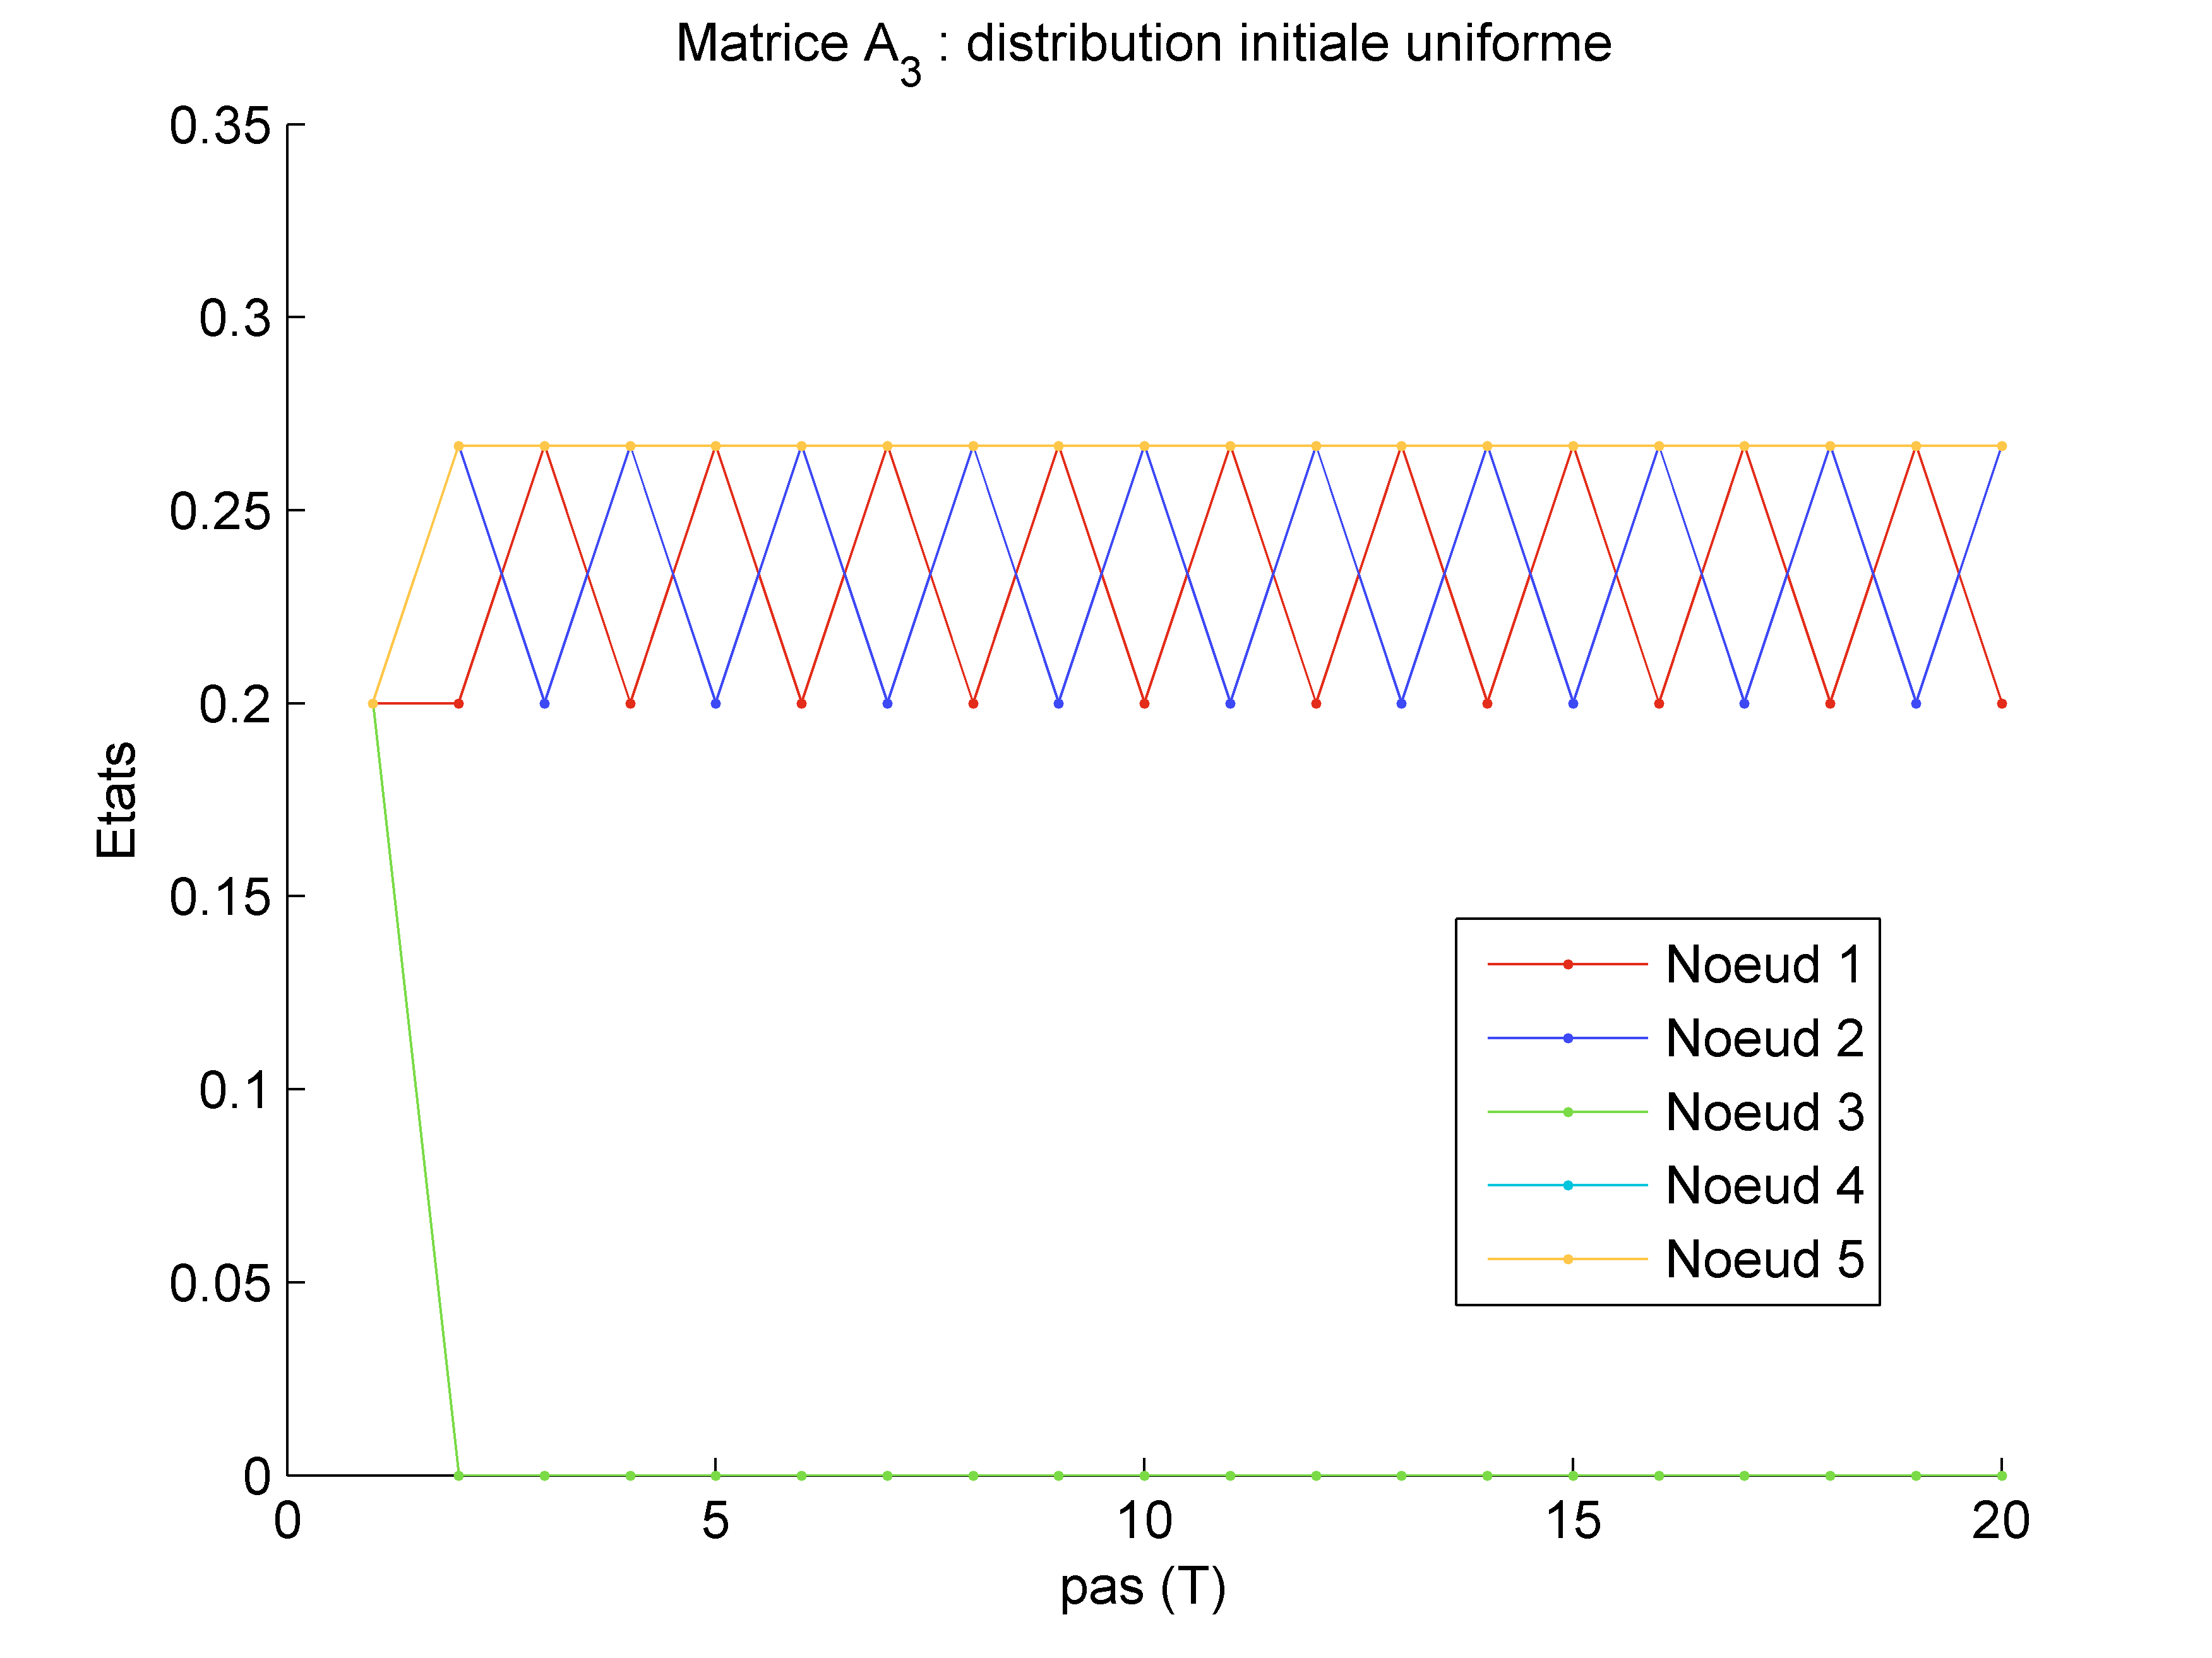
\includegraphics[scale=0.45]{../images/q118_evol_31.png}\label{sfig:q118_evol}}
	\subfigure[Depuis le noeud 1]{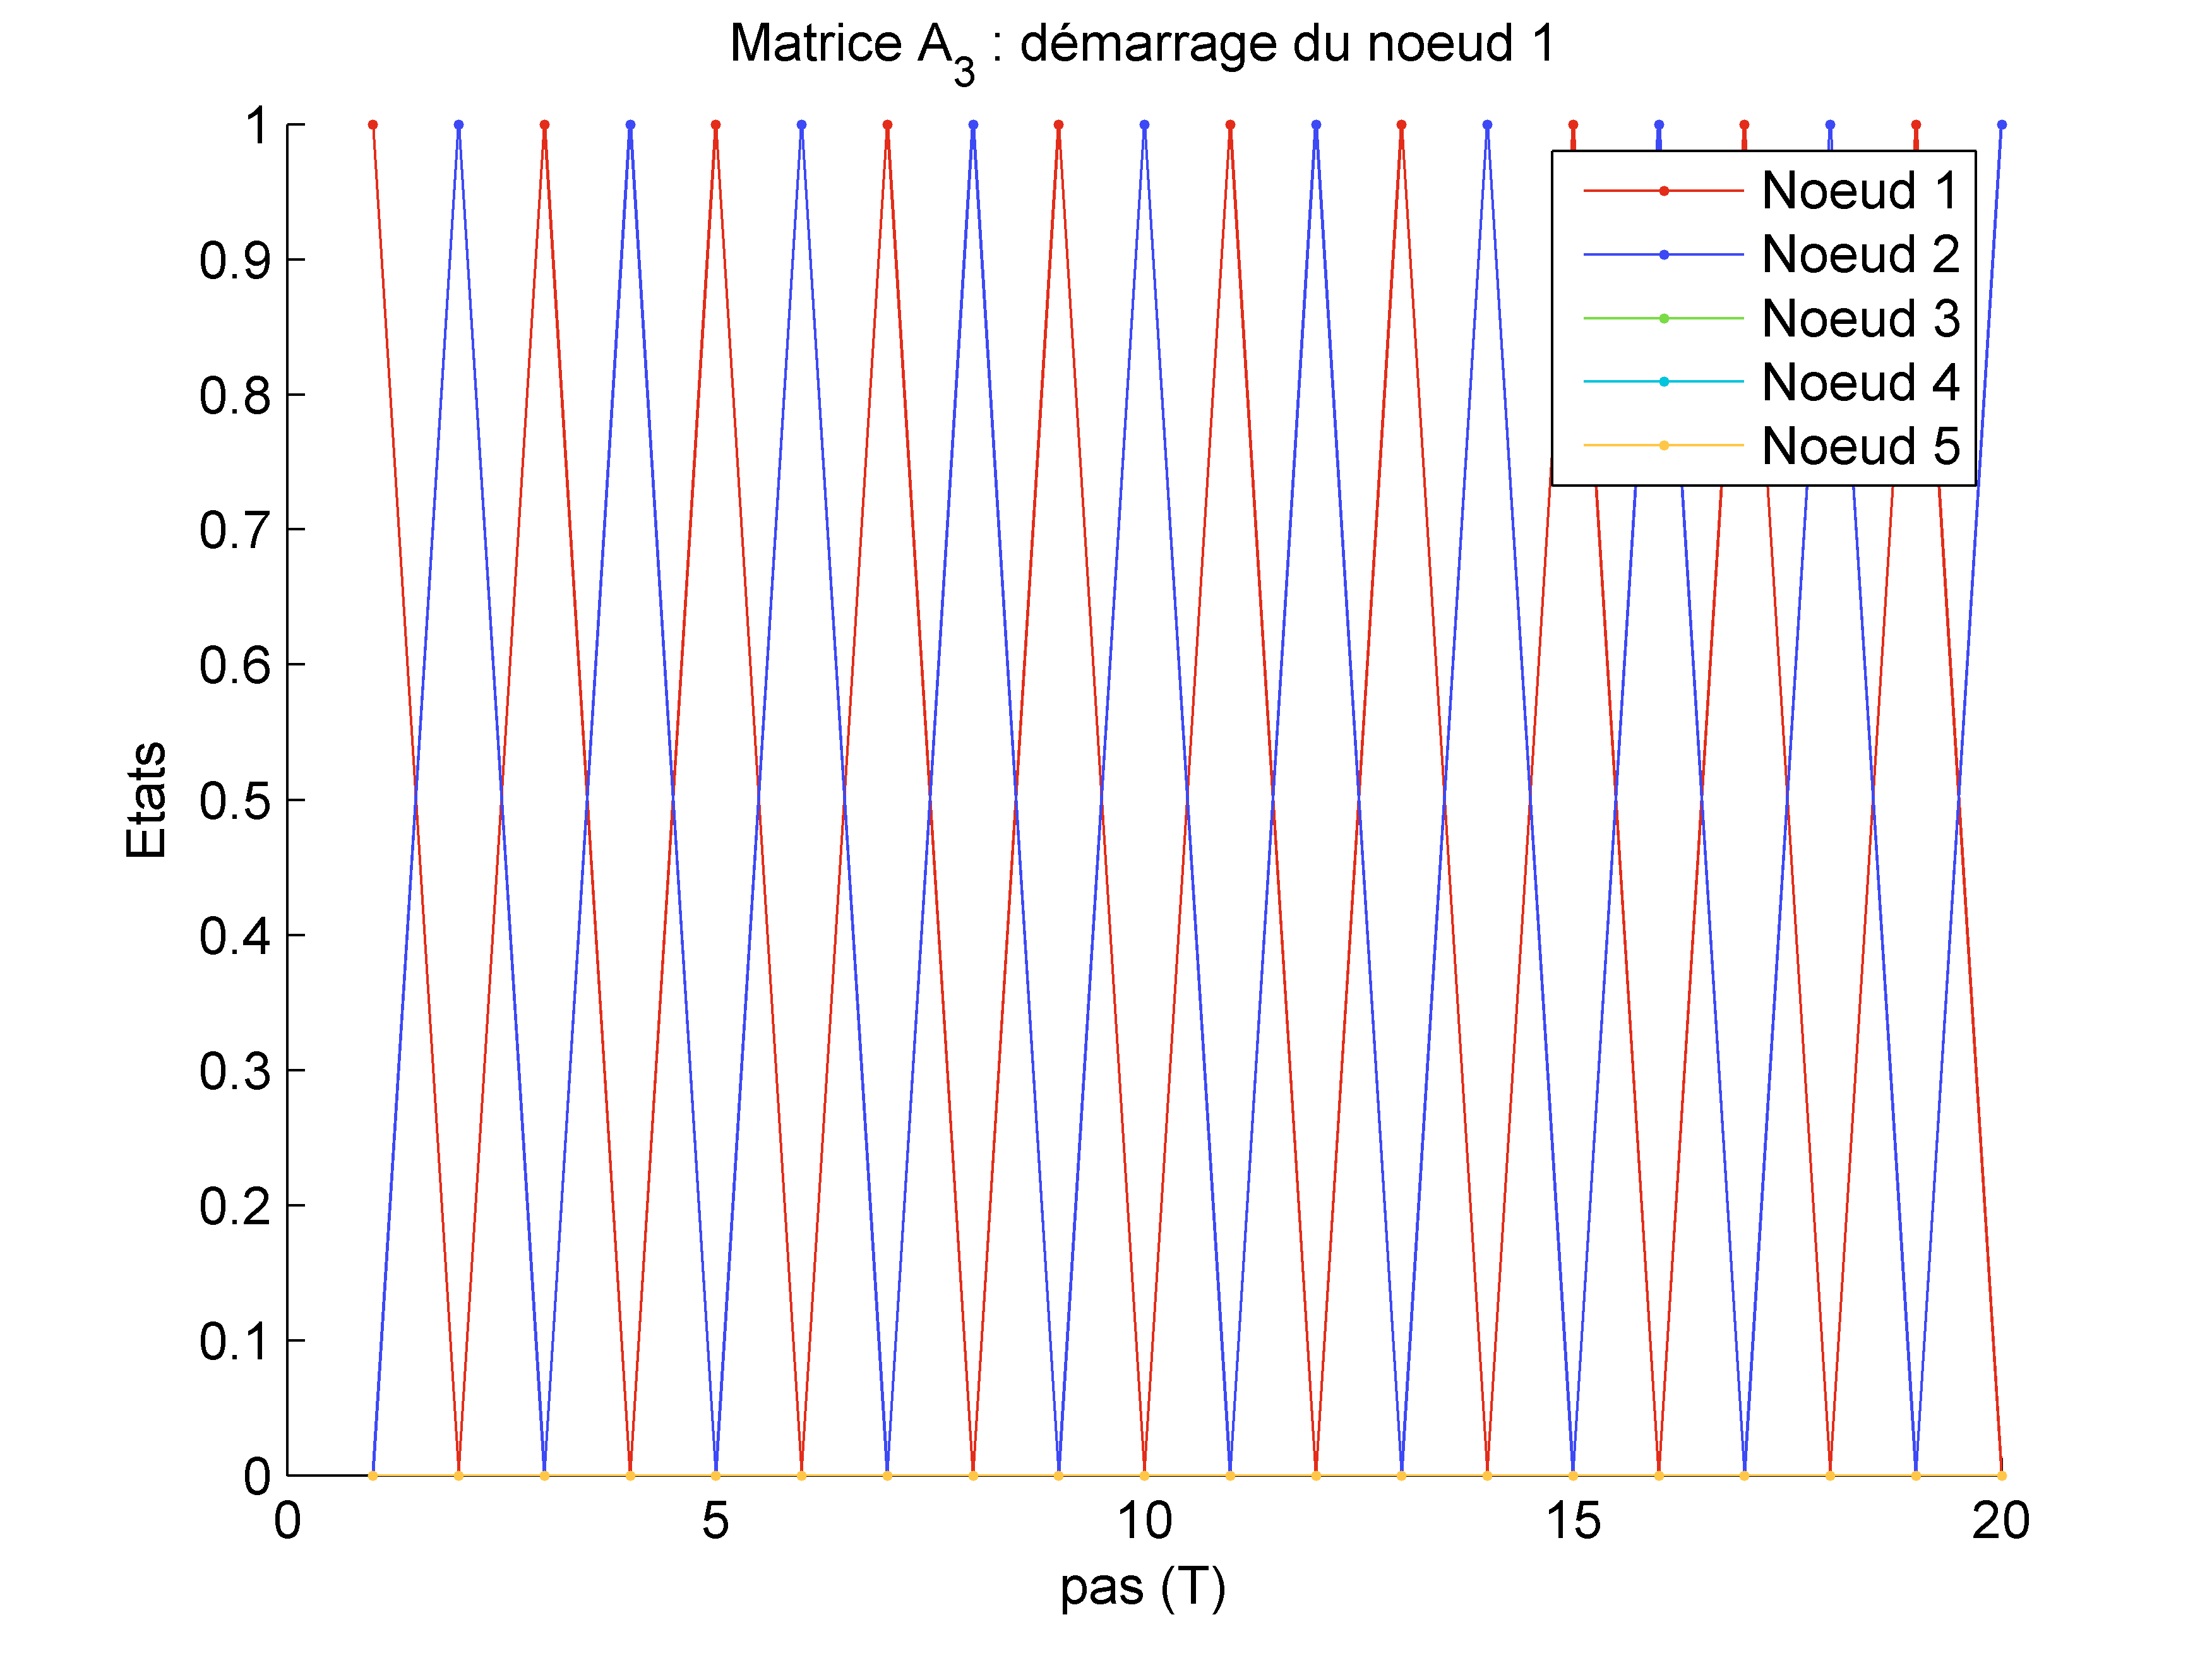
\includegraphics[scale=0.45]{../images/q118_evol_32.png}\label{sfig:q118_evol}}
	\caption{Évolution des distributions de probabilités}
	\label{fig:q118}
\end{figure}

\paragraph{2)} Tout d'abord, affichons les résultats obtenus à partir de la fonction \texttt{findStationnaryPi} (\textit{cfr.} question 1.1.4 - méthode des puissances) appliquée aux différentes matrices de transition : 
\begin{center}
	\begin{tabular}{c|ccccc}
		& Nœud 1 & Nœud 2 & Nœud 3 & Nœud 4 & Nœud 5\\
		\hline
		$Q_1$ & $0.3750$ & $0.1875$ & $0.1875$ & $0.2500$ & ---\\
		$Q_2$ & $0.3750$ & $0.3750$ & $0$ & $0.2500$ & ---\\
		$Q_3$ & $0.2667$ & $0.2000$ & $0$ & $0.2667$ & $0.2667$\\  
	\end{tabular}
\end{center}
Notons que les distributions pour $Q_2$ et $Q_3$ ont été calculés à partir d'une distribution uniforme.
\paragraph{}
Dans cette section, deux méthodes de calcul ont été utilisées : 
\begin{itemize}
	\item \textbf{Résolution du système linéaire} : On a $\pi_{\infty} Q = \pi_{\infty}$ et $\sum_i \pi_{\infty, i} = 1$, que l'on peut transformer en un système : 
	\[
		\begin{aligned}
			(Q' - \mathbb{1}) \pi^T_{\infty} = b
		\end{aligned}
	\]
	où $Q'$ est formé de la matrice $Q^T$ à laquelle une ligne de `$1$' a été ajoutée (matrice de taille $(k+1) \times k$, $k$ étant le nombre de nœuds) et $b$ est un vecteur colonne (de taille $k+1$) composé de zéros sauf le dernier élément qui vaut `$1$'.
	\item \textbf{Résolution par vecteurs/valeurs propres} : On a le système suivant : 
	\[
		\begin{aligned}
			\pi_{\infty} Q &= \pi_{\infty}\\
			\Leftrightarrow Q^T \pi^T_{\infty} &= \pi^T_{\infty}
		\end{aligned}
	\]
	Cette équation est une équation de type $Ax = \lambda x$, où $A$ est de taille $n\times n$, x est $n\times 1$ et $\lambda$ est un scalaire. Ce type d'équation est en fait un calcul de recherche de vecteurs et valeurs propres. Dans notre cas, la valeur propre $\lambda$ vaut 1, il s'agit alors de calculer le vecteur propre correspondant et de le normaliser afin de respecter l'équation $\sum_i \pi_{\infty, i} = 1$, ce qui a été implémenté dans la fonction \texttt{getStationnaryPiBySystem}.
\end{itemize}
\paragraph{}
Ces deux méthodes donnent un résultat exactement identique pour chaque matrice de transition, à l'exception du troisième graphe pour lequel une distribution supplémentaire a été trouvée. En effet, la fonction \texttt{linsolve} émet un warning ``\textit{Rank deficient}'' nous informant que le système est indéterminé, il n'y a pas suffisamment d'équations - rang de $Q' - \mathbb{1}$ < nombre d'inconnues, mais ne renvoie qu'une seule solution. On peut en déduire qu'il existe une infinité de solutions.
\paragraph{}
On peut obtenir ce même résultat à partir des deux distributions obtenues par la méthode des vecteurs/valeurs propres : supposons les distributions stationnaires $\pi_A$ et $\pi_B$, par définition : 
\[
	\pi_A Q_3 = \pi_A
\]
et
\[
	\pi_B Q_3 = \pi_B
\]
On peut alors trouver une autre distribution (stationnaire) qui est combinaison des deux précédentes :
\[
	(\alpha\pi_A + \beta\pi_B) Q_3 = (\alpha\pi_A + \beta\pi_B)
\]
On peut en déduire qu'il existe une infinité de distributions stationnaires pour la matrice $Q_3$.
\paragraph{}
Contrairement à la matrice $A_1$, les matrices $A_2$ et $A_3$ ne donnent pas le même résultats qu'avec la fonction \texttt{findStationnaryPi}. En effet, en exécutant celle-ci, le message ``\textit{Number of maximum iterations reached}'' apparaît, signifiant que la sortie a une plus forte probabilité d'être un état non-stationnaire, c'est-à-dire que la fonction a été arrêtée avant d'atteindre un état stationnaire (s'il y en a un par la suite). Dans notre cas, en affichant les distributions, on peut voir que celles-ci sont périodiques, cela étant du aux cycles présents dans les graphes.
\paragraph{}
Concernant le deuxième graphe, le système d'équation est déterminé (rang de $Q' - \mathbb{1}$ = nombre d'inconnues), le vecteur que l'on obtient est bien unique. On peut observer que la probabilité de passer par le nœud 3 est nulle, nous sommes en effet en présence d'un graphe réductible. Au vu de la propriété des distributions stationnaires, nous continuerons dans l'état stationnaire si la distribution initiale est la distribution stationnaire. De même pour le troisième graphe, nous continuerons dans l'état stationnaire si la distribution initiale est une des distributions stationnaires.

\section{Téléportation}
\label{sec:teleport}
\paragraph{1)}
La formule utilisée pour calculer la matrice de transition $Q_t$ du modèle du surfeur avec téléportation est la suivante :
\[
	Q_t = (1 - \alpha) Q' + \alpha \tilde{Q}
\]
où $Q'$ et $\tilde{Q}$ sont des matrices de transition et $\alpha$ la probabilité de téléportation. 
\paragraph{}
La première est la matrice de transition du graphe initial auquel on a rajouté des arêtes partant des \textit{dangling nodes}. Elle a été calculée en remplaçant par $\frac{1}{n}$ tous les éléments de la matrice $Q$ situés dans des lignes ne contenant que des 0. Cette valeur $\frac{1}{n}$ a été choisie en considérant une densité de probabilité uniforme entre les différentes arêtes partant des \textit{dangling nodes}. 
\paragraph{}
La seconde est la matrice de transition d'un graphe complet formé à partir des nœuds du graphe initial. Il s'agit, autrement dit, de la matrice de transition représentant la téléportation. Une combinaison linéaire de paramètre $\alpha$ est ensuite appliquée aux deux matrices pour trouver la matrice $Q_t$.
\paragraph{2)}
On sait qu'une distribution stationnaire $\pi_s$ est unique si \textbf{la chaîne de Markov est irréductible}. Autrement dit, il faut que pour tout couple de nœuds $(i_1$, $i_2)$, il existe une arête les reliant (un probabilité non-nulle de passer de $i_1$ à $i_2$). Cette propriété est vérifiée avec le modèle du surfeur modifié puisque la téléportation permet, depuis tout nœud, de se diriger vers un autre nœud tant que $\alpha > 0$. 
\paragraph{}
A partir du moment où $\alpha = 0$, on n'est plus assuré que chaque paire de nœuds est reliée par une arête et donc que $\pi_s$ est bien stationnaire.
\paragraph{3)} 
Le classement des sites les plus visités, obtenus à l'aide de la distribution stationnaire, est donné dans la Table \ref{tab:best_page_rank}.
\begin{table}[h]
	\center
	\begin{tabular}{|c|c|c|}
		\hline
		N\degre & PageRank & Page \\
		\hline
		1 & 0.0045 & http://purl.org/rss/1.0/modules/content \\
		2 & 0.0027 & http://www.ulg.ac.be \\
		3 & 0.0024 & http://ogp.me/ns$\sharp$ \\
		4 & 0.0024 & http://www.gre-liege.be  \\
		5 & 0.0023 & http://blog.intelliterwal.net  \\
		6 & 0.0023 & http://www.jalios.com  \\
		7 & 0.0022 & http://www.vmfnet.be  \\
		8 & 0.0022 & http://www.alinoa.be  \\
		9 & 0.0022 & http://www.ulb.ac.be  \\
		10 & 0.0022 & http://www.cedia.ulg.ac.be  \\
		\hline
	\end{tabular}
	\caption{Classement des sites ayant le meilleur PageRank ($\alpha = 0.15$)}
	\label{tab:best_page_rank}
\end{table}
\paragraph{4)}
Soit $ X_{t_j}$ la variable aléatoire qui prend la valeur $p_i$ au temps $t_j$ si le surfeur est sur la page i.
On veut calculer : $$
P(X_{t_2} = p_2 | X_{t_3} = p_3 , X_{t_1} = p_1)
$$
En appliquant la formule de Bayes et en se rappelant de la propriété d'une chaîne de Markov, on obtient :
$$ \dfrac{P(X_{t_2} = p_2 | X_{t_1} = p_1) \cdot P(X_{t_3} = p_3 | X_{t_2} = p_2,)}{P(X_{t_3} = p_3 | X_{t_1} = p_1)} $$

Lorsque l'on passe à la notation matricielle, on a :

$$\dfrac{Q^{t_3 - t_2}(p_3, p_2) \cdot Q^{t_2 - t_1}(p_2, p_1)}{Q^{t_3 - t_1}(p_3, p_1)}
$$

Enfin en appliquant la formule pour le cas désigné dans l'énoncé, nous obtenons :

$$\dfrac{Q^{10}(p_3, p_2) \cdot Q^{9}(p_2, p_1)}{Q^{19}(p_3, p_1)} = 0.0308
$$

\section{Effet du $\alpha$}
\label{sec:effet_alpha}
\paragraph{1)}
Pour prouver que le score PageRank de toute page est au moins $\frac{\alpha}{n}$ ($n$ est le nombre de pages), on peut développer une expression ``\textit{explicite}'' des éléments de la matrice $Q_t$ en utilisant la formule donnée précédemment : 
\[
Q_t(i,j) = q_{ij} (1 - \alpha) + \dfrac{1}{n}\alpha\\
\]
où $q_{ij}$ est un élément de la matrice $Q'$. Connaissant la relation qui lie $\pi^{(k)}$ et $\pi^{(k-1)}$, on a :
\[
\begin{aligned}
\pi^{(k)}_j &= \sum\limits_{i = 1}^n Q_t(i,j)\pi^{(k-1)}_i\\
 &= \sum\limits_{i = 1}^n \left(q_{ij} (1 - \alpha) + \dfrac{\alpha}{n}\right)\pi^{(k-1)}_i\\
 &= \sum\limits_{i = 1}^n q_{ij} (1 - \alpha) \pi^{(k-1)}_i + \sum\limits_{i = 1}^n \dfrac{\alpha}{n} \pi^{(k-1)}_i\\
 &= \dfrac{\alpha}{n} + \underbrace{(1 - \alpha) \sum\limits_{i = 1}^n q_{ij} \pi^{(k-1)}_i}_{> 0}
\end{aligned}
\]
Le deuxième terme est inférieur à 1 (et même inférieur à $(1 - \frac{\alpha}{n})$ afin de respecter le deuxième axiome de Kolmogorov) et surtout, positif. De ce fait, on peut affirmer que :
\[
\pi^{(k)}_j \geq \dfrac{\alpha}{n}
\]
On peut interpréter le cas où $\alpha = 0$ comme le cas où il n'y a pas de téléportation et le cas où $\alpha = 1$ comme le cas où il n'y a que téléportation (le surfeur n'utilise plus que les liens). Remarquons les valeurs prises par les distributions dans les deux cas :
\[
\begin{array}{l}
\pi_{\alpha = 0}^{(k)} = \pi^{(k-1)} Q'\\ \\
\pi_{j,\alpha = 1}^{(k)} = \frac{1}{n}, \forall j
\end{array}
\]
\paragraph{}
Dans le deuxième cas, les PageRank de toutes les pages seront égaux et vaudront $\frac{1}{n}$. Afin de vérifier cette affirmation, nous avons calculé la distribution stationnaire pour $\alpha = 1$ et l'avons mise en parallèle avec la distribution stationnaire pour $\alpha = 0.15$. Le résultat est édifiant (voir Table \ref{tab:alpha_comp}), on constate en effet un PageRank uniforme dans le cas où $\alpha = 1$ .
\begin{table}[h]
	\center
	\begin{tabular}{|c|c|c|}
		\hline 
		$\alpha$   & 0.15  & 1 \\
		\hline
	 	Moyenne    & 0.002 & 0.002\\
	 	Ecart-type & 1.3000e-04 & \textbf{4.7753e-18} \\
	 	Min.       & 0.0019 & 0.002\\
	 	Max.       & 0.0045 & 0.002\\
	 	\hline
	\end{tabular}
	\caption{Statistiques à propos des distributions stationnaires avec $\alpha = 0.15$ et $\alpha = 1$}
	\label{tab:alpha_comp}
\end{table}
\paragraph{2)}
Nous avons analysé l'évolution du PageRank de certaines pages lorsque alpha évolue. En regardant la Figure \ref{sfig:evolPageRankAlpha}, on observe que plus alpha est grand, plus le PageRank des pages tend à s'uniformiser. En effet, un PageRank élevé au départ va diminuer avec l'augmentation de $\alpha$, tandis qu'un PageRank assez bas va augmenter avec $\alpha$ vu que plus alpha est élevé, plus la probabilité d'arriver sur une telle page s'uniformise.   

\begin{figure}[h]
	\center
	\subfigure{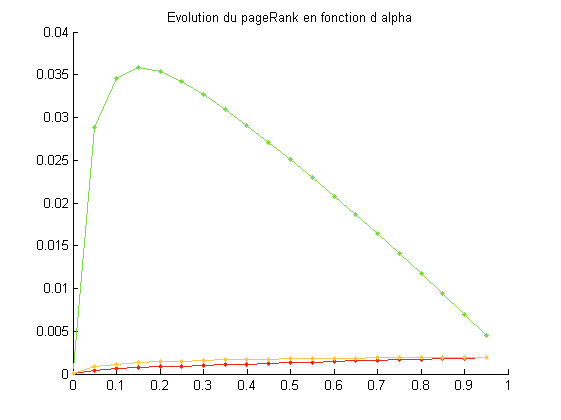
\includegraphics[scale=0.47]{../images/evolPagerank.png}\label{sfig:evolPageRankAlpha}}
	\subfigure{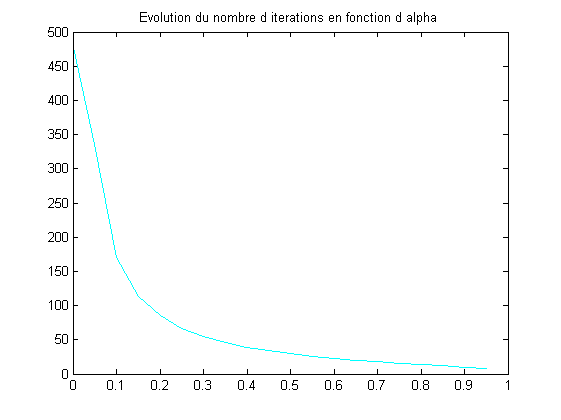
\includegraphics[scale=0.47]{../images/nbItAlpha.png}\label{sfig:nbItAlpha}}
	\caption{Évolution du PageRank et du nombre d'itérations avec $\alpha$}
\end{figure}
\paragraph{3)}
Nous avons déterminé l'évolution du nombre d'itérations nécessaires pour trouver une distribution stationnaire lorsque $\alpha$ varie. Les résultats sont présentés sur la Figure \ref{sfig:nbItAlpha}.
\paragraph{}
Les résultats observés sont attendus car il est logique de trouver une distribution stationnaire très rapidement lorsque $\alpha$ tend vers 1, étant donné que on ne tient compte que de la téléportation: la probabilité d'arriver sur une page ou une autre partant d'une page donnée est uniforme. Dans le cas contraire, lorsque alpha tend vers zéro, on ne repose plus sur le graphe de départ ce qui est plus compliqué à calculer qu'une répartition uniforme.


\chapter{Question 2}
\section{Estimation d'une matrice de transition}
\label{sec:estimateQ}
\subsection{Méthode d'estimation}
Avant tout, voici les quelques notations que nous utiliserons : 
\begin{itemize}
	\item $n$, le nombre de noeuds dans le graphe
	\item $X$, la trace fournie (chaîne de Markov)
	\item $Q_{est}$, la matrice de transition recherchée
	\[
		Q_{est} = 
		\begin{pmatrix}
			\theta_{11} & \cdots & \theta_{1n}\\
			\vdots & \ddots & \vdots\\
			\theta_{n1} & \cdots & \theta_{nn}\\
		\end{pmatrix}
	\]
	\item $N$, la matrice dont l'élément $\beta_{ij}$ est le nombre de transition de l'état $i$ à $j$ dans la trace $X$
	\item $\sigma_i$, la somme de la $i^{\text{ème}}$ ligne de la matrice $N$
	\item $\underline{\theta}_i$, le vecteur contenant les probabilités pour passer du nœud $i$ à un autre nœud : 
	\[
		\underline{\theta}_i = [\theta_{i1} \cdots \theta_{in}]
	\]
	\item $P(X|\underline{\theta}_i)$, la probabilité d'observer les départs du nœud $i$ présents dans la trace connaissant $\underline{\theta}_i$ :
	\[
		P(X|\underline{\theta}_i) = \theta_{i1}^{\beta_{i1}} \times \cdots \times \theta_{i(n - 1)}^{\beta_{i(n - 1)}} \times \left(1 - \sum\limits_{k = 1}^{n - 1} \theta_{ik}\right)^{\beta_{in}} = \left(1 - \sum\limits_{k = 1}^{n - 1} \theta_{ik}\right)^{\beta_{in}} \times \prod\limits_{k = 1}^{n - 1} \theta_{ik}^{\beta_{ik}}
	\]
	\item $S_i$, le système de $n - 1$ équations à résoudre pour trouver la ligne $i$ de la matrice de transition par la méthode du maximum de vraisemblance. On note $S_{ij}$ la $j^{\text{ième}}$ équation de ce système :
	\[
		S_i \equiv 
		\left\{
		\begin{array}{c}
		\dfrac{\partial P(X|\underline{\theta}_i)}{\partial \theta_{i1}} = 0\\
		\vdots\\
		\dfrac{\partial P(X|\underline{\theta}_i)}{\partial \theta_{i(n-1)}} = 0\\
		\end{array}
		\right.
	\] 
	La résolution de ce système ne donne que les $n-1$ probabilités de la ligne $i$. Il suffit de les sommer pour obtenir la $n^{\text{ième}}$.
\end{itemize}
\paragraph{}
Développons l'équation trouvée ci-dessus (pour $j \in [2, n-2]$ mais que l'on peut facilement généraliser pour les cas où $j = 1$ ou $(n-1)$):

\[
	\begin{aligned}
		S_{ij} &= \left[\beta_{ij} \theta_{ij}^{\beta_{ij} - 1} \left(1 - \sum\limits_{k = 1}^{n - 1} \theta_{ik}\right)^{\beta_{in}} - \beta_{in} \left(1 - \sum\limits_{k = 1}^{n - 1} \theta_{ik}\right)^{\beta_{in} - 1} \theta_{ij}^{\beta_{ij}}\right] \times \prod\limits_{k = 1, k \neq j}^{n - 1} \theta_{ik}^{\beta_{ik}}\\
		&= \left[\beta_{ij}  \left(1 - \sum\limits_{k = 1}^{n - 1} \theta_{ik}\right) - \beta_{in}  \theta_{ij}\right]\times \left(1 - \sum\limits_{k = 1}^{n - 1} \theta_{ik}\right)^{\beta_{in} - 1} \times \theta_{ij}^{\beta_{ij} - 1} \times \prod\limits_{k = 1, k \neq j}^{n - 1} \theta_{ik}^{\beta_{ik}} = 0\\
	\end{aligned}
\]
Il nous reste à résoudre l'équation suivante :
\[
	\begin{aligned}
		&\beta_{ij} \left(1 - \sum\limits_{k = 1}^{n - 1} \theta_{ik}\right) - \beta_{in} \theta_{ij} = 0\\
		\Leftrightarrow \text{ }&\beta_{ij} \left(1 - \sum\limits_{k = 1}^{n - 1} \theta_{ik}\right) = \beta_{in} \theta_{ij}\\
		\Leftrightarrow \text{ }& \dfrac{\beta_{in}}{\beta_{ij}} \theta_{ij} + \sum\limits_{k = 1}^{n - 1} \theta_{ik} = 1\\
		\Leftrightarrow \text{ }& \left(\dfrac{\beta_{in}}{\beta_{ij}} + 1\right) \theta_{ij} + \sum\limits_{k = 1, k \neq j}^{n - 1} \theta_{ik} = 1 \text{ } (1)	
	\end{aligned}
\]
Le système $S_i$ peut se réécrire sous forme matricielle de la manière suivante : 
\[
S_i \equiv 
\begin{pmatrix}
\left(\dfrac{\beta_{in} + \beta_{i1}}{\beta_{i1}}\right) & 1 & \cdots & 1 \\
1 & \ddots &  \ddots & \vdots \\
\vdots &  \ddots & \ddots & 1\\
1 & \cdots & 1   & \left(\dfrac{\beta_{in} + \beta_{i(n - 1)}}{\beta_{i(n - 1)}}\right)
\end{pmatrix}
\begin{pmatrix}
\theta_{i1}\\
\vdots\\
\theta_{i(n - 1)}
\end{pmatrix}
= 
\begin{pmatrix}
1\\
\vdots\\
1\\
\end{pmatrix}
\]
La résolution de ce système pour chaque ligne permet d'obtenir une estimation de la matrice de transition. Néanmoins, cette méthode est extrêmement inefficace puisqu'elle nécessite $n$ résolutions du système. Bien qu'à notre échelle ($n = 50$), cette complexité élevée ne soit pas gênante, une simplification de la méthode d'estimation serait tout de même la bienvenue. 
\paragraph{}
Repartons de l'équation $(1)$ : 
\[
\begin{aligned}
	&\left(\dfrac{\beta_{in}}{\beta_{ij}} + 1\right) \theta_{ij} + \sum\limits_{k = 1, k \neq j}^{n - 1} \theta_{ik} = 1\\
	&\Leftrightarrow \dfrac{\beta_{in}}{\beta_{ij}} \theta_{ij} + \theta_{ij} = 1 - \sum\limits_{k = 1, k \neq j}^{n - 1} \theta_{ik}\\
	&\Leftrightarrow \dfrac{\beta_{in}}{\beta_{ij}} \theta_{ij} + \theta_{ij} = \theta_{ij} + \theta_{in}\\
	&\Leftrightarrow \theta_{ij}= \dfrac{\theta_{in}}{\beta_{in}} \beta_{ij}\text{ }(2)\\
	&\Leftrightarrow \sum\limits_{i = 0}^{n - 1} \theta_{ij} = \dfrac{\theta_{in}}{\beta_{in}} \sum\limits_{i = 0}^{n - 1}\beta_{ij}\\
	&\Leftrightarrow 1 - \theta_{in} = \dfrac{\theta_{in}}{\beta_{in}} \left(\sigma_i - \beta_{in}\right)\\	
	&\Leftrightarrow \theta_{in} = \dfrac{\beta_{in}}{\sigma_{i}} \text{ }(3)\\	
\end{aligned}
\]
\paragraph{}
En injectant l'équation $(3)$ dans l'équation $(2)$, on obtient l'équation :
\[
\theta_{ij} = \dfrac{\beta_{ij}}{\sigma_{i}}
\]
\paragraph{}
La formule ci-dessus nous permet de simplifier l'estimation puisque qu'il suffit maintenant de \textbf{diviser chaque élément $\beta_{ij}
$ de la matrice $N$ par la somme de la ligne dans laquelle il se trouve} pour trouver la matrice de transition. Il ne reste plus qu'à régler le problème où
\[
\beta_{ij} = 0, \forall j \in [1,n]
\]
En effet, cette situation mènerait à une division par zéro. Il faut donc appliquer un traitement à la matrice $N$ afin de supprimer les valeurs nulles.

\subsubsection{Smoothing}
Un des problèmes liés à l'estimation par le maximum de vraisemblance se pose lorsque le set de données permettant d'estimer $Q$ ne contient pas d'information sur certains nœuds, \textit{i.e.} $\beta_{ij} = 0$. En effet, lorsque par la suite, nous souhaiterions estimer la probabilité qu'une certaine séquence, contenant un nœud qui n'a pas été compté pour estimer $Q$, corresponde à ce modèle, nous obtiendrons une probabilité nulle.
\paragraph{}
Plusieurs techniques de lissage existent : soient la transition du nœud $\omega_{i-1}$ vers le nœud $\omega_i$ observée, $c(x)$ le nombre de fois où le nœud $x$ a été compté, $c(x,y)$ le nombre de fois la transition du nœud $x$ vers le nœud $y$ a été compté et $n$ le nombre de nœuds : \\
\begin{itemize}
	\item \textbf{Méthode de Laplace (\textit{Laplace smoothing}) :} Cette méthode consiste à ajouter 1 à tous les éléments comptés. On obtient alors une probabilité de la forme : 
	\[
		P_{Laplace} (\omega_i | \omega_{i-1}) = \frac{c(\omega_{i-1}, \omega_i) + 1}{c(\omega_{i-1}) + n}
	\]
	\item \textbf{\textit{Add-k smoothing} :} Cette méthode généralise la méthode de Laplace où, cette fois, $k$ est ajouté au numérateur et $k.n$ est ajouté au dénominateur : 
	\[
		P_{Add-k} (\omega_i | \omega_{i-1}) = \frac{c(\omega_{i-1}, \omega_i) + k}{c(\omega_{i-1}) + k.n}
	\]
	\item \textbf{\textit{Unigram prior smoothing} :} Il s'agit d'une variante de l'\textit{add-k smoothing} où la probabilité d'obtenir le noeud (unigramme) $\omega_i$ intervient. Par rapport à la formule de l'\textit{add-k smoothing}, on prend $k = m/n$ où $m$ est un paramètre à déterminer. On obtient alors : 
	\[
		P_{Add-k-var} (\omega_i | \omega_{i-1}) = \frac{c(\omega_{i-1}, \omega_i) + m . \left(\frac{1}{n}\right)}{c(\omega_{i-1}) + m}
	\]
	La ``subtilité'' de l'\textit{unigram prior smoothing} consiste à remplacer la constante $\frac{1}{n}$ au numérateur par $P(\omega_i)$. On a au final : 
	\[
	\begin{aligned}
		P_{UnigramPrior} (\omega_i | \omega_{i-1}) 
			&= \frac{c(\omega_{i-1}, \omega_i) + m . P_{ML}(\omega_i)}{c(\omega_{i-1}) + m}\\
			&= \frac{c(\omega_{i-1}, \omega_i) + m \frac{c(\omega_i)}{n}}{c(\omega_{i-1}) + m}\\
	\end{aligned}
	\]
	\item \textbf{\textit{Jelinek-Mercer smoothing} (interpolation) :} Il s'agit d'une interpolation linéaire entre le modèle de l'unigramme (noeud) et du bigramme (transitions) afin de pouvoir prendre en compte les probabilités de ces deux modèles : 
	\[
	\begin{aligned}
		P_{Jelinek-Mercer} (\omega_i | \omega_{i-1}) 
			&= \lambda . P_{ML}(\omega_i | \omega_{i-1}) + (1 - \lambda) . P_{ML}(\omega_i)\\
			&= \lambda \frac{c(\omega_i, \omega_{i-1})}{c(\omega_i)} + (1 - \lambda) \frac{c(\omega_i)}{n}
	\end{aligned}
	\]	
\end{itemize}
Il existe encore d'autres méthodes que nous n'avons pas implémentées : \\
\begin{itemize}
	\item \textbf{\textit{Good-Turing} : } Cette méthode agit sur les éléments non vus (transitions ne figurant pas dans la trace) et rectifie ce compte en fonction des éléments comptés 1 fois, 2 fois,... Les transitions effectuées $r$ fois seront modifiés en $r^*$ tel que $r^* = (r+1) \frac{n_{r+1}}{n_r}$, où $n_r$ est le nombre de transitions comptés exactement $r$ fois.
\end{itemize}

\subsection{Utilisation des modèles estimés}
\label{ssec:util_esti}
Une méthode pour déterminer l'origine des traces d'un ensemble de traces consiste à calculer la probabilité $P(Q_i|tr_k)$ que $tr_k$ provienne d'une certaine matrice de transition $Q_i$ (la matrice de transition définissant le comportement d'un surfeur). Il suffira ensuite de prendre le surfeur dont la matrice de transition mène à la plus grande probabilité. Autrement dit : 
\[
arg \max\limits_i P(Q_i|tr_k)
\]
À l'aide de la formule de Bayes, on peut développer : 
\[
P(Q_i|tr_k) = \dfrac{P(tr_k|Q_i) P(Q_i)}{\sum\limits_{j = 1}^n P(tr_k|Q_j) P(Q_j)}
\]
où le terme $P(tr_k|Q_i)$ est la vraisemblance de la trace connaissant la matrice $Q_i$ et $P(Q_i)$ est la probabilité qu'une trace provienne du surfeur $i$.
\paragraph{}
Dans notre cas, la vraisemblance est un nombre tellement petit qu'il n'est pas représentable sur un ordinateur (à moins d'utiliser des bibliothèques spéciales). Nous avons donc décidé d'utiliser la \textbf{log-vraisemblance} de sorte que les nombres soient manipulables. 
\paragraph{} 
Étant donné que les traces $tr_k$ ne peuvent appartenir qu'à deux surfeurs, nous pouvons aussi modifier notre règle de décision. Pour ce faire, nous définissons le \textit{log-ratio} :
\[
\begin{aligned}
r &= \log \dfrac{P(Q_1|tr_k)}{P(Q_2|tr_k)}\\
&= \log \dfrac{P(tr_k|Q_1) P(Q_1)}{P(tr_k|Q_2) P(Q_2)}\\
&= \log P(tr_k|Q_1) - \log P(tr_k|Q_2) + \log \dfrac{P(Q_1)}{P(Q_2)}
\end{aligned}
\]
Si $r > 0$ alors la trace d'origine provient du \textbf{surfer 1} sinon elle provient du \textbf{surfer 2}. Notons que dans notre cas :
\[ 
	P(Q_i) = \frac{1}{2}, \forall i \in [1,2]
\]
En effet, nous savons que parmi les 20 traces à évaluer, 10 appartiennent au premier (soit la moitié) et 10 au deuxième (soit l'autre moitié).  
\subsubsection{Calcul de la vraisemblance}
Pour une trace $X$, une matrice $N$ contenant les éléments $\beta_{ij}$ (nombre de transitions de l'état $i$ à $j$ dans $X$) et une matrice de transition $Q$, la vraisemblance est donnée par : 
\[
P(X|Q) = \prod\limits_{i = 1}^n \prod\limits_{j = 1}^n \theta_{ij}^{\beta_{ij}}
\]
Comme expliqué plus haut, nous utiliserons la log-vraisemblance qui se calcule comme suit :
\[
log P(X|Q) = \sum\limits_{i = 1}^n\sum\limits_{j = 1}^n \beta_{ij} \log \theta_{ij}
\]

\subsection{Analyse des 20 traces}
En appliquant la méthode expliquée dans la Section \ref{ssec:util_esti}, nous avons obtenu les résultats donnés dans la Table \ref{tab:surf_trace}. Pour la raison expliquée précédemment, nous ne savons pas calculer explicitement la probabilité $ P(Q_i|tr_k)$. Nous avons néanmoins donné le \textit{log-ratio} $r$ qui est, dans ce cas ci, la différence entre les log-vraisemblances.
Nous observons bien 10 traces provenant du premier surfeur et 10 traces provenant du second.
\begin{table}[ht]
	\center
	\begin{tabular}{|c|cc|}
		\hline
		Trace & $r$ & Provient de \\
		\hline
		1 & $ -0.4361$ & $\mathbf{2}$ \\
		2 & $57.737$ & $\mathbf{1}$ \\
		3 & $70.562$ & $\mathbf{1}$ \\
		4 & $68.022$ & $\mathbf{1}$ \\
		5 & $-153.35$ & $\mathbf{2}$ \\
		6 & $127.45$ & $\mathbf{1}$ \\
		7 & $-47.847$ & $\mathbf{2}$ \\
		8 & $47.912$ & $\mathbf{1}$ \\
		9 & $-13.472$ & $\mathbf{2}$ \\
		10 & $-10.209$ & $\mathbf{2}$ \\
		11 & $-183.48$ & $\mathbf{2}$ \\
		12 & $-155.67$ & $\mathbf{2}$ \\
		13 & $52.513$ & $\mathbf{1}$ \\
		14 & $10.682$ & $\mathbf{1}$ \\
		15 & $19.723$ & $\mathbf{1}$ \\
		16 & $-104.7$ & $\mathbf{2}$ \\
		17 & $-34.937$ & $\mathbf{2}$ \\
		18 & $12.536$ & $\mathbf{1}$ \\
		19 & $-53.645$ & $\mathbf{2}$ \\
		20 & $126.89$ & $\mathbf{1}$ \\
		\hline
	\end{tabular}
	\caption{Recherche des surfeur ayant engendré les traces}
	\label{tab:surf_trace}
\end{table}
\subsection{Hypothèses, fiabilité et limites}
Pour appliquer la méthode du maximum de vraisemblance, on doit uniquement connaître les probabilités qui nous sont données par le graphe. Nous avons testé les résultats de notre méthode. 

\subsubsection{Test de la méthode}
Pour tester cette méthode, nous avons procédé en plusieurs étapes : 
\begin{enumerate}
	\item Définition d'une matrice d'adjacence $A$ de taille $k \times k$ (ici, $k = 5$)
	\item Calcul de la matrice de transition $Q$ et génération de $n$ (ici, $n = 50$) chaînes de Markov $X_i$ de taille $m$ (ici, $m = 1000$)
	\item Génération de $n$ estimations $Q_{est,i}$ de la matrice de transition sur base des chaînes générées (méthode de lissage : \textit{add-k} avec $k = 0.06$)
	\item Calcul du module du biais $E$ pour chaque $\theta_{ij}$ 
\end{enumerate}
\paragraph{}
En utilisant cette méthode nous avons obtenu des résultats intéressants. Ci-dessous sont donnés la matrice $Q$ exacte, le biais moyen sur les $50$ générations et $Q_{est}$, une des matrices estimées :
\[
Q = 
\begin{pmatrix}
 0.1 & 0.1 & 0.1 & 0.1 & 0.6\\
 0.1 & 0.1 & 0.1 & 0.35 & 0.35\\
 0.1 & 0.35 & 0.1 & 0.35 & 0.1\\
 0.6 & 0.1 & 0.1 & 0.1 & 0.1\\
 0.35 & 0.1 & 0.35 & 0.1 & 0.1 
\end{pmatrix}
\]
\[
E = 
\begin{pmatrix}
0.0011 & 0.0006 & 0.0006 & 0.0005 & 0.0044\\
0.0021 & 0.0006 & 0.0009 & 0.0039 & 0.0020\\
0.0022 & 0.0035 & 0.0006 & 0.0027 & 0.0020\\
0.0067 & 0.0007 & 0.0007 & 0.0007 & 0.0017\\
0.0015 & 0.0006 & 0.0017 & 0.0005 & 0.0009 
\end{pmatrix}
\]
\[
Q_{est} = 
\begin{pmatrix}
0.1309 & 0.1078 & 0.1106 & 0.1112 & 0.5396\\
0.1413 & 0.1072 & 0.1191 & 0.3047 & 0.3276\\
0.1431 & 0.2986 & 0.1140 & 0.3043 & 0.1400\\
0.5221 & 0.1076 & 0.1174 & 0.1176 & 0.1353\\
0.3301 & 0.1110 & 0.3157 & 0.1167 & 0.1265\\
\end{pmatrix}
\]
Cette configuration nous a donné un biais moyen de $0.0318$.

\paragraph{} Étudions maintenant l'évolution du biais en fonction de $m$, la taille des traces. Pour ce faire, nous fixons $k$ et $n$ à 50. Ensuite, pour chaque valeur de $m$, nous appliquons la méthode de test expliquée ci-dessus et récupérons la moyenne et l'écart type du biais que nous portons sur le graphe. La \textsc{Figure} \ref{fig:evol_m_bias} montre les courbes obtenues. Nous constatons (et c'était attendu) que le biais induit par l'estimation diminue lorsque la taille de la trace augmente.
\begin{figure}[h]
	\center
	\subfigure[{\textit{add-$\lambda$ smoothing} : $\lambda = 1$}]{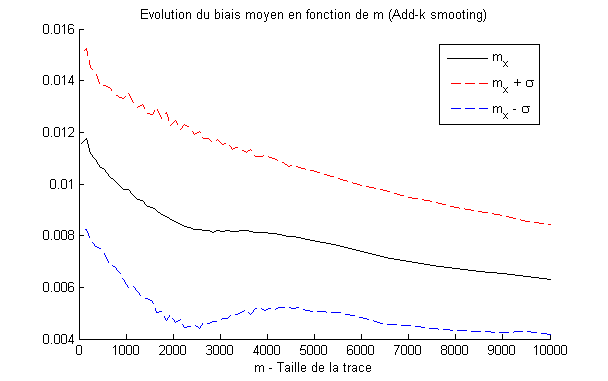
\includegraphics[scale=0.45]{../images/evol_m_bias_AK1_E.png}}
	\subfigure[{\textit{add-$\lambda$ smoothing} : $\lambda = 0.06$}]{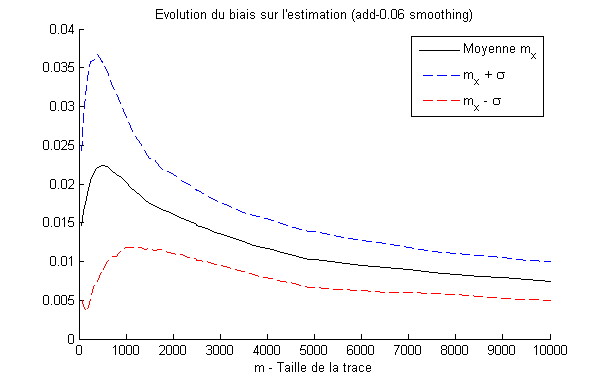
\includegraphics[scale=0.45]{../images/evol_m_bias_AK006_E.png}}
	\caption{Évolution du biais moyen en fonction de la taille des chaînes de Markov}
	\label{fig:evol_m_bias}
\end{figure}
\paragraph{}
Notons que la méthode de \textit{smoothing} influe grandement sur cette courbe. En effet, on peut constater la présence d'un maximum dans l'intervalle $m \in [0,1000]$ dans le cas du \textit{add-$0.06$ smoothing}. La zone où se trouve ce maximum est particulière puisque elle correspond à une chaîne relativement courte comparée au nombre de transitions possibles (ici, $2500$) sur le graphe. De ce fait, elle n'est pas assez représentative du surfeur. 
\subsection{Applications possibles de la méthode}
Les chaînes de Markov ont de nombreuses applications possibles dans des domaines très variés tels que les sciences sociales, la biologie, les sciences économiques et pleins d'autres. \\ \\

Pour citer quelques exemples, on utilise les modèles de Markov pour identifier les régions de l'ADN génomique qui codent les gènes, pour la reconnaissance et la synthèse vocale, pour prédire les éruptions d'un geyser et bien d'autres encore. \\ \\

 Dans notre parcours universitaire, nous avons déjà utilisé un modèle de Markov caché pour définir une caractéristique d'un texte (langue, auteur). L'algorithme se basait sur plusieurs échantillons de textes ayant des caractéristiques différentes. Nous établissions des modèles sur base de ces échantillons et testions ensuite l'appartenance d'un texte à l'un des modèles. Grâce à cet algorithme, nous avons pu discerner la langue d'un texte, le langage d'un code, l'auteur d'un livre à partir d'échantillons pour chaque caractéristique. Malgré la simplicité de ce programme, nous pouvions déjà faire un certain nombre de tests différents. 

\section{Estimation de $\alpha$}
\subsection{Méthodes d'estimation}
\subsubsection{Méthode algébrique}
\paragraph{1)} Le paramètre $\alpha$ est un paramètre de la matrice de transition représentant un surfeur aléatoire. Nous avons défini dans la Section \ref{sec:effet_alpha}, la formule définissant chaque élément de cette matrice de transition en fonction de $\alpha$ pour le modèle du surfeur aléatoire : 
\[
Q_t(i,j) = q_{ij} (1 - \alpha) + \dfrac{\alpha}{n}\\
\]
Un approche algébrique consiste à utiliser cette formule afin de définir $\alpha$. En effet, en isolant le paramètre, on obtient :
\[
	\alpha = \dfrac{Q_t(i,j) - q_{ij}}{\frac{1}{n} - q_{ij}}
\]
\paragraph{}
Regardons de plus près cette formule : 
\begin{itemize}
	\item $q_{ij}$ : puisque nous connaissons le graphe parcouru par le surfeur, nous connaissons ce terme de manière exacte (voir Section \ref{sec:teleport})
	\item $Q_t(i,j)$ : ce terme provient de la matrice de transition du surfeur. Celle-ci est inconnue puisque nous recherchons son paramètre $\alpha$. Nous pouvons néanmoins l'estimer en utilisant la méthode du maximum de vraisemblance (voir Section \ref{sec:estimateQ}). L'erreur d'estimation induite par cette estimation se propagera dans la valeur calculée de $\alpha$.
	\item Si $q_{ij} = \frac{1}{n}$ : notre formule nous donne alors un $\alpha$ infini. Ce cas correspond à la situation où le noeud $i$ est un \textit{dangling node}. Si ce cas se présente, il faut donc éliminer les résultats correspondants.
\end{itemize} 
\paragraph{}
Finalement, nous disposons de $n^2$ équations qui nous fournissent un échantillon d'au plus $n^2$ estimations. L'estimateur de $\alpha$ peut être trouvé en prenant la moyenne de cet échantillon. 
\paragraph{}
Nous avons implémenté cette méthode et l'avons testée d'abord sur notre propre jeu de données. En l'occurrence, nous avons utilisé une matrice d'adjacence d'ordre 7. Nous l'avons ensuite testée (en appliquant la méthode expliquée dans la Section 2.3) sur les 22 traces fournies et avons trouvé des résultats cohérents. 
\paragraph{} 
Nous avons enfin voulu appliquer un test final qui consistait à évaluer la qualité des estimations pour des variations de paramètres et nous avons commencé par une variation du paramètre $k$, l'ordre du graphe. Nous avons alors remarqué un gros défaut de notre méthode qui est mis en évidence sur la Figure \ref{fig:alpha_horrible}. L'erreur commise s'accroît très rapidement quand le paramètre $k$ augmente ce qui rend inutilisable notre méthode pour des grands graphes. Après avoir effectué ces observations, nous avons cherché une autre méthode d'estimation. 
\begin{figure}[ht]
	\center
	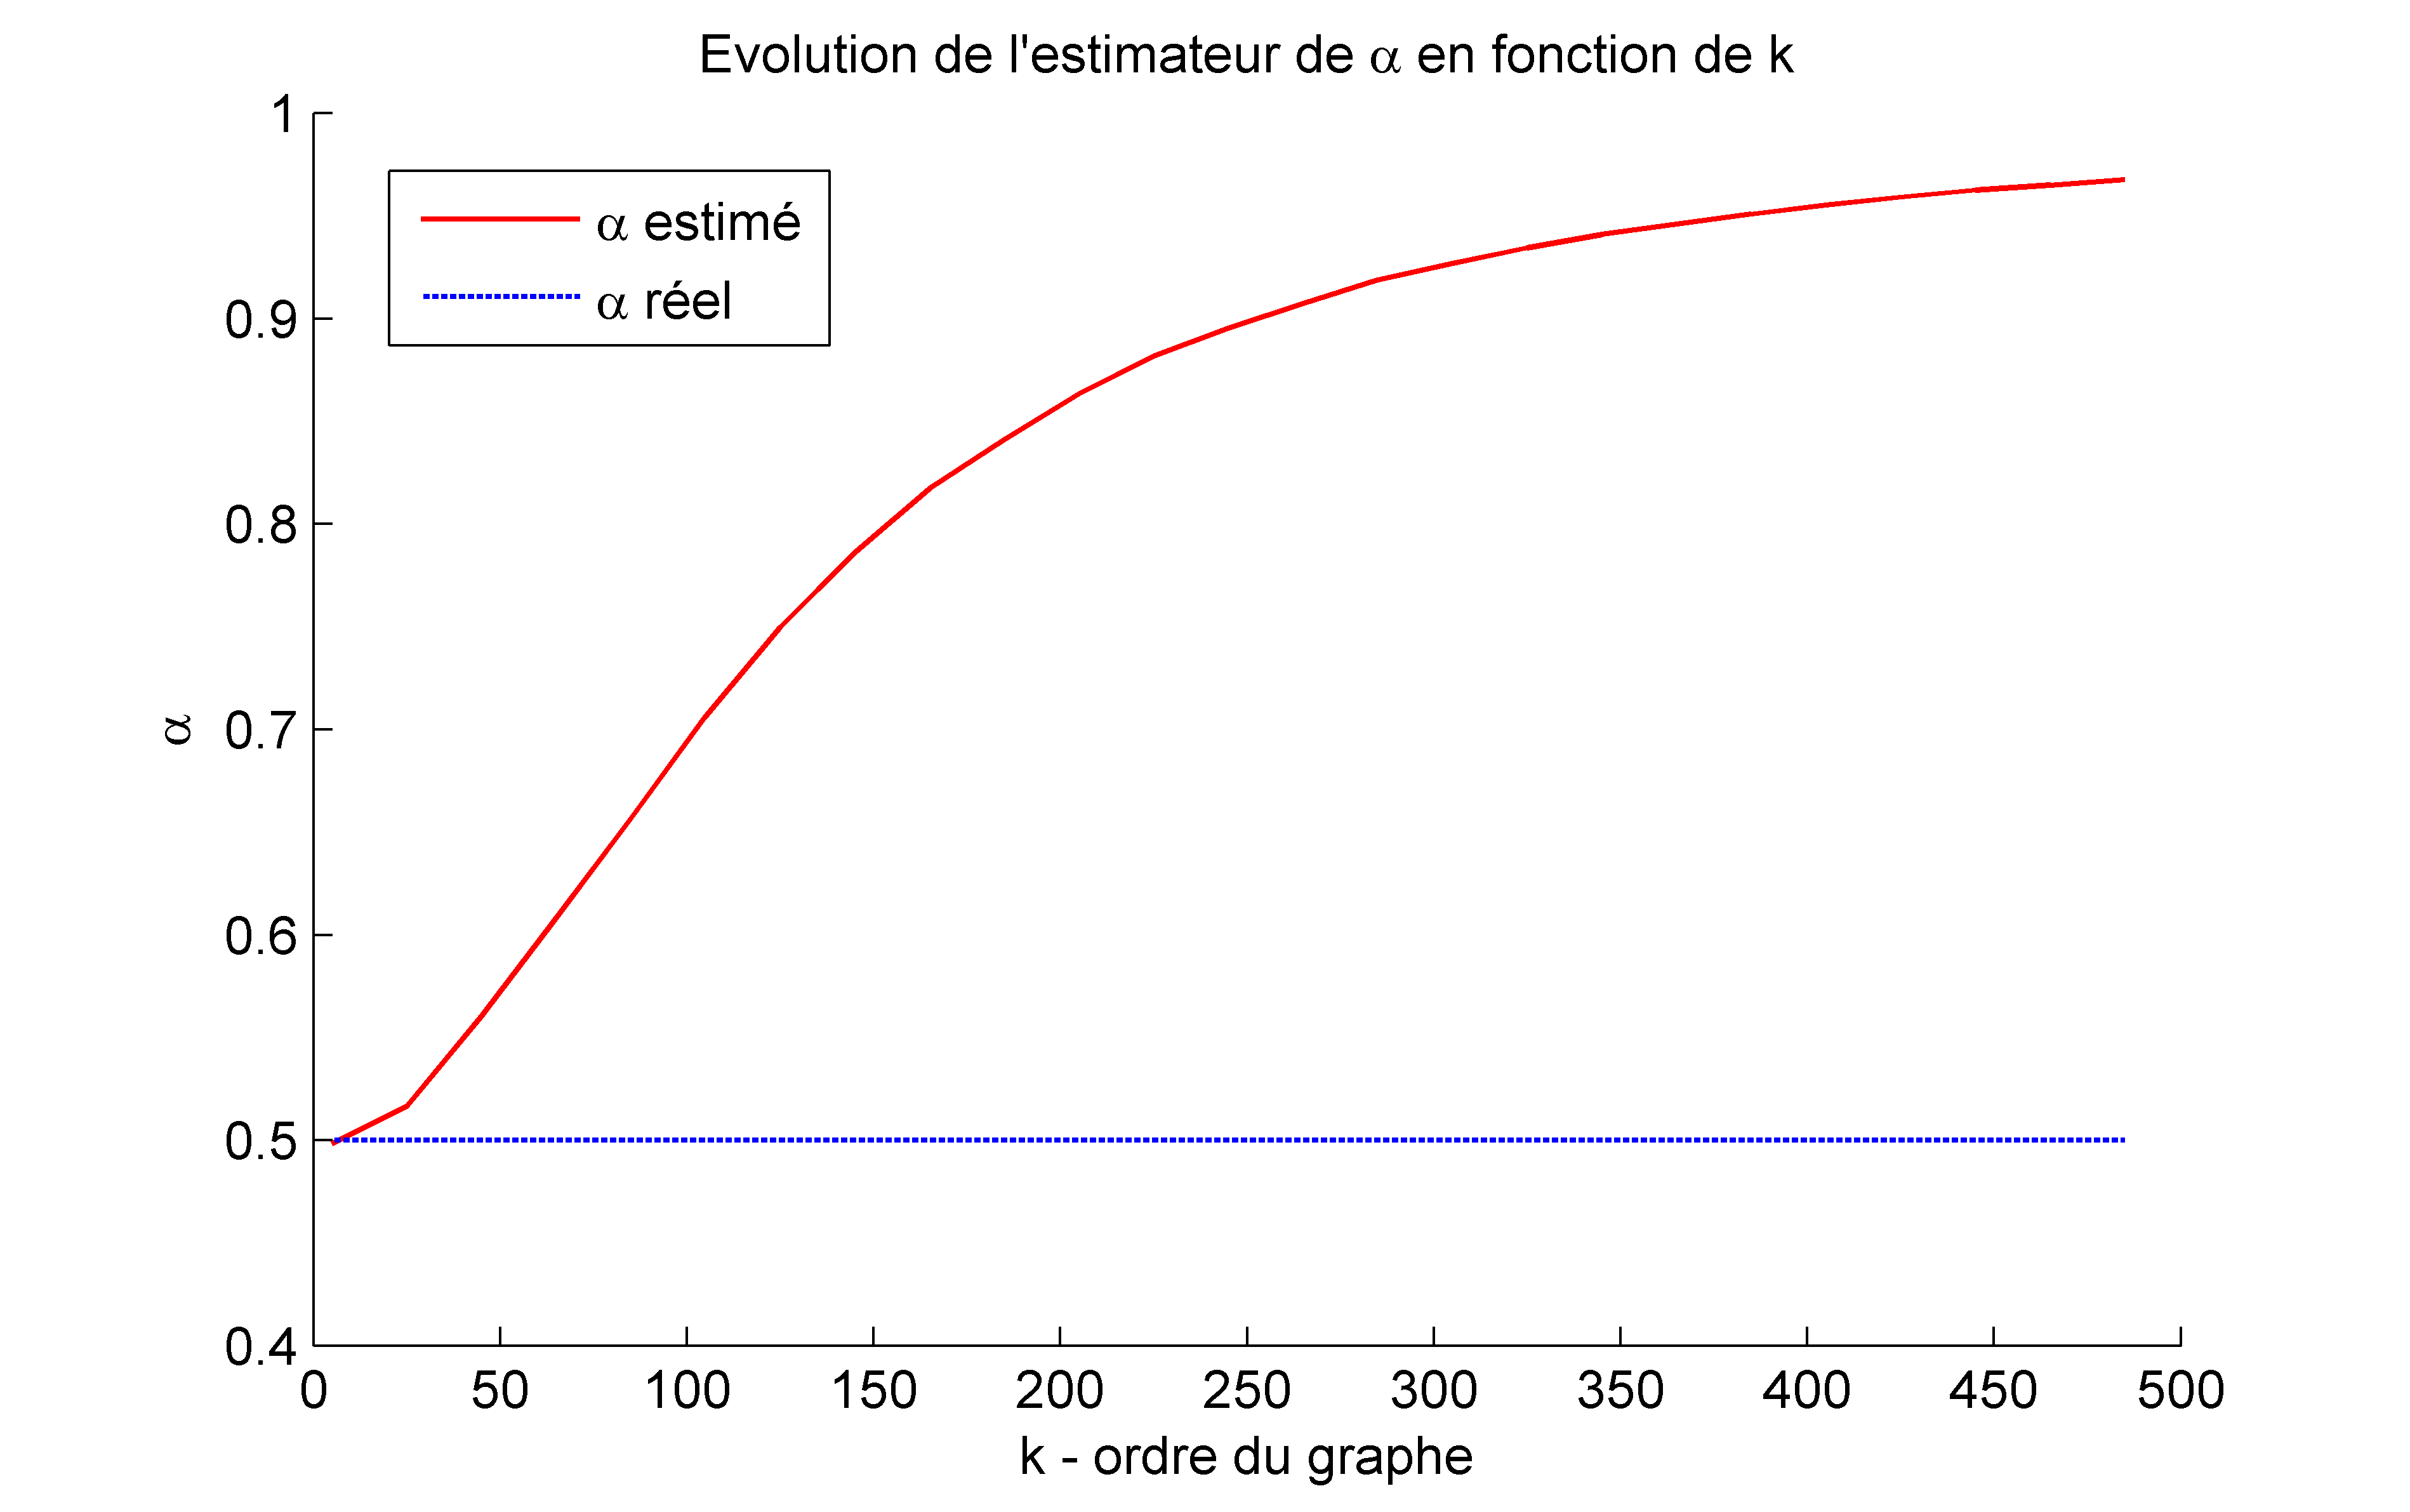
\includegraphics[scale=0.5]{../images/alpha_horrible.png}
	\caption{Évolution de $\alpha$ en fonction de $k$ - Méthode algébrique}
	\label{fig:alpha_horrible}
\end{figure}
\subsubsection{Par le maximum de vraisemblance}
Cette méthode consiste à générer la valeur de $\alpha$ qui maximise la vraisemblance d'une trace. Dans le cas où nous nous intéressons à $n$ traces, nous procédons de la manière suivante : 
\begin{itemize}
	\item Nous générons un vecteur $v$ contenant des valeurs de $\alpha$ couvrant l'intervalle $[0,1]$ (de la manière suivante :  \texttt{0.01:step:1})
	\item Pour chaque $\alpha_i$ de $v$, nous générons la matrice de transition $Q_i$ correspondante (prenant en compte la téléportation) 
	\item Nous calculons la log-vraisemblance de chaque trace pour chaque matrice et nous sélectionnons le $\alpha_i$ qui a mené à la plus grande log-vraisemblance pour chaque trace.
\end{itemize}
\paragraph{}
Cette méthode, bien que satisfaisante du point de vue des résultats qu'elle fournit, est loin d'être efficace. En effet, nous devons générer une grand nombre de matrices de transition (ce nombre étant fonction du pas \texttt{step} appliqué) puis calculer la log-vraisemblance de toutes les traces pour toutes ces matrices. L'algorithme pourrait être amélioré en utilisant des méthodes d'optimisation numérique qui permettraient de ne pas devoir calculer toutes les matrices de transitions mais uniquement certaines d'entre elles. Nous pourrions aussi passer par développement analytique de la formule du maximum de vraisemblance. Ce développement pourrait mener, comme ce fût le cas dans la Section \ref{sec:estimateQ} pour l'estimation de $Q$, à une autre méthode plus efficace et plus simple.

\section{Identification de l'origine d'une trace}
Pour définir l'appartenance d'une trace à l'un des deux modèles, nous estimons la valeur des $\alpha_i$ des traces $Tr_i$ des surfeurs grâce à la méthode décrite au premier point et nous considérons que une trace ayant un $\alpha$ estimé appartient au surfeur ayant un $\alpha_i$ le plus proche.

\section{Application aux 20 traces}
Nous avons calculé les valeurs de $\alpha$ pour chaque surfeur.

\begin{center}
	\begin{tabular}{c|l}
		$S_1$ & 0.4010\\
		$S_2$ & 0.6030\\
	\end{tabular}
\end{center}
                                 
\begin{table}[h]
	\center
	\begin{tabular}{c|c|c}
		Trace & $\alpha$ & Méthode $\alpha$\\
		\hline
		1 & 0.4120 &  1  \\
		2 & 0.4060 & 1 \\
		3 & 0.6320 & 2 \\ 
		4 & 0.3790 & 1 \\
		5 & 0.5870 & 2 \\
		6 & 0.3430 & 1 \\
		7 & 0.6350 & 2 \\
		8 & 0.4030 & 1 \\
		9 & 0.5610 & 2 \\
		10 & 0.5880 & 2 \\
		11 & 0.6450 & 2 \\
		12 & 0.6140 & 2 \\
		13 & 0.4250 & 1 \\
		14 & 0.3880 & 1 \\
		15 & 0.4120 & 1 \\
		16 & 0.6370 & 2 \\
		17 & 0.3860 & 1 \\
		18 & 0.5400 & 2 \\
		19 & 0.6070 & 2 \\
		20 & 0.4070 & 1 \\
	\end{tabular}
	\caption{Identification de l'origine des traces}
\end{table}

 Si on compare avec le tableau \ref{tab:surf_trace}, on remarque que 4 estimations diffèrent : celles pour les traces 1, 3, 17 et 18. Au vu des résultats des tests de nos méthodes, nous aurions plus tendance à choisir l'estimation à partir de $\alpha$ car l'erreur est plus faible.
 
\section{Estimer $Q$ sans connaître le graphe ni $\alpha$}
Dans la section 2.1, nous utilisons uniquement la trace et l'ordre du graphe pour générer la matrice de transition Q. Une idée est donc de réutiliser cette méthode, mais seulement en remplaçant l'ordre du graphe par le nombre d'états distincts dans la trace. Nous créons donc un modèle de Markov caché car certains états peuvent être inconnus. Cette approximation devrait être correcte lorsque la taille de la trace est suffisamment grande de sorte que la plupart des états soient représentés dans celle-ci. Par contre si la trace est petite ou ne montre pas un nombre suffisant d'état, les résultats seraient très mauvais.

\appendix

\chapter{Comparaison de différentes méthodes de lissage}


\section{Estimation de $Q$}
	\subsection{Évolution de l'erreur en fonction de la taille de la trace}

On compare ici les précisions atteignables par les différentes méthodes, en comparant les erreurs quadratiques réalisées par rapport à $Q$ lors de la modifications de paramètres relatifs à ces méthodes. Le graphe utilisé est le graphe donné dans l'énoncé.

\paragraph{}
La \textsc{Table A.1} reprend les erreurs à paramètres fixés pour différentes tailles $m_t$ de la trace. On peut remarquer que les méthodes ``\textit{add-k}'' et ``\textit{unigram prior}'' donnent des résultats fortement semblables, leurs précisions augmentent de la même façon. En comparaison avec l'interpolation, celle-ci possède une décroissance nettement plus faible, malgré le fait qu'elle possède une erreur quadratique plus grande pour des plus petites traces. 
\begin{table}[h]
	\center
	\begin{tabular}{c|ccc}
	$m_t$ & Add-k ($k = 0.06$) & Unigram prior ($m = 0.06 * 50$) & Interpolation ($\lambda = 0.3$)\\
	\hline
	100 & \num{0.0013755} & \num{0.0015444} & \num{0.00042131}\\
	300 & \num{0.0014585} & \num{0.0014937} & \num{0.00028596}\\
	500 & \num{0.0011939} & \num{0.0012146} & \num{0.00025819}\\
	800 & \num{0.00090119} & \num{0.00091241} & \num{0.00024232}\\
	1000 & \num{0.00076995} & \num{0.00077718} & \num{0.00022381}\\
	2000 & \num{0.00043842} & \num{0.00043775} & \num{0.00022826}\\
	5000 & \num{0.00018841} & \num{0.00018972} & \num{0.00022237}\\	
	10000 & \num{0.000096356} & \num{0.000096745} & \num{0.00022023}\\	
	\end{tabular}
	\caption{Précision de l'estimation de $Q$}
	\label{tab:}
\end{table}

\subsection{Détermination des paramètres minimisant l'erreur}

La \textsc{Table A.2} reprend les différentes précisions obtenues en modifiant le paramètre $k$ de la méthode ``\textit{add-k}'', avec une taille de trace fixée à 5000. On remarque ici que la valeur minimale se situe en $\lambda = 1$.
\begin{table}[h]
	\center
	\begin{tabular}{c|c}
		$\lambda$ & ``\textit{Add-k}''\\
		\hline
		0.02 & \num{0.000205509}\\
		0.04 & \num{0.000206059}\\
		0.06 & \num{0.000199354}\\
		0.08 & \num{0.000192963}\\
		0.1 & \num{0.000194727}\\
		0.3 & \num{0.000158402}\\
		0.5 & \num{0.000140448}\\
		0.7 & \num{0.000128312}\\
		0.9 & \num{0.00011945}\\
		1 & \num{0.000117869}
	\end{tabular}
	\caption{Estimation du paramètre $k$ pour la méthode \textit{add-k}}
\end{table}

\paragraph{}
La \textsc{Table A.3} reprend les différentes précisions obtenues en modifiant le paramètre $m$ de la méthode ``\textit{uniform prior}'', avec une taille de trace fixée à 5000. On remarque ici que la valeur minimale se situe en $m = 100$.

\begin{table}[h]
	\center
	\begin{tabular}{c|c|c}
		$k$ & $m = k . 50$ & Unigram prior\\
		\hline
		0.01 & 0.5 & \num{0.00019824}\\
		0.1 & 5 & \num{0.00018813}\\
		0.3 & 15 & \num{0.00015445}\\
		0.5 & 25 & \num{0.00013759}\\
		0.7 & 35 & \num{0.00012522}\\
		0.9 & 45 & \num{0.00011752}\\
		1 & 50 & \num{0.00011499}\\
		2 & 100 & \num{0.00010787}\\
		3 & 150 & \num{0.0001149}\\
		5 & 250 & \num{0.000133235}
	\end{tabular}
	\caption{Estimation du paramètre $m$ pour la méthode ``\textit{uniform prior}''}
\end{table}

\paragraph{}
La \textsc{Table A.4} reprend les différentes précisions obtenues en modifiant le paramètre $\lambda$ de la méthode par interpolation, avec une taille de trace fixée à 5000.

\begin{table}[h]
	\center
	\begin{tabular}{c|c}
		$\lambda$ & Interpolation\\
		\hline
		0.1 & \num{0.00022511}\\
		0.2 & \num{0.00022374}\\
		0.3 & \num{0.00022222}\\
		0.4 & \num{0.00022023}\\
		0.5 & \num{0.000219}\\
		0.6 & \num{0.00021351}\\
		0.7 & \num{0.00020713}\\
		0.8 & \num{0.00020226}\\
		0.9 & \num{0.00016776}\\
		1 & \num{0.00019933}
	\end{tabular}
	\caption{Estimation du paramètre $\lambda$ pour la méthode par interpolation}
\end{table}

\begin{thebibliography}{9}

\bibitem{NLP}
  Bill MacCartney,
  \emph{NLP Lunch Tutorial: Smoothing}.
  \url{http://nlp.stanford.edu/~wcmac/},
  21 Avril 2005.

\bibitem{ProbEst}
  D. De Cao, R. Basili,
  \emph{Probability Estimation}.
  23 Avril 2009.

\bibitem{Est-MLE-S}
  David Smith,
  \emph{Estimation - Maximum likelihood and smoothing} (Introduction to Natural Language Processing course). University of Massachusetts Amherst,
  Fall 2009.

\bibitem{Craven}
  Dr. Mark Craven,
  \emph{Markov Chain Models}

\bibitem{coursea}
 \url{https://www.coursera.org/course/nlp}

\bibitem{staskexchange}
  \href{http://stats.stackexchange.com/questions/47685/calculating-log-likelihood-for-given-mle-markov-chains}{http://stats.stackexchange.com/.../calculating-log-likelihood-for-given-mle-markov-chains}
\end{thebibliography}

\end{document}
